% Options for packages loaded elsewhere
\PassOptionsToPackage{unicode}{hyperref}
\PassOptionsToPackage{hyphens}{url}
%
\documentclass[
  ignorenonframetext,
]{beamer}
\usepackage{pgfpages}
\setbeamertemplate{caption}[numbered]
\setbeamertemplate{caption label separator}{: }
\setbeamercolor{caption name}{fg=normal text.fg}
\beamertemplatenavigationsymbolsempty
% Prevent slide breaks in the middle of a paragraph
\widowpenalties 1 10000
\raggedbottom
\setbeamertemplate{part page}{
  \centering
  \begin{beamercolorbox}[sep=16pt,center]{part title}
    \usebeamerfont{part title}\insertpart\par
  \end{beamercolorbox}
}
\setbeamertemplate{section page}{
  \centering
  \begin{beamercolorbox}[sep=12pt,center]{part title}
    \usebeamerfont{section title}\insertsection\par
  \end{beamercolorbox}
}
\setbeamertemplate{subsection page}{
  \centering
  \begin{beamercolorbox}[sep=8pt,center]{part title}
    \usebeamerfont{subsection title}\insertsubsection\par
  \end{beamercolorbox}
}
\AtBeginPart{
  \frame{\partpage}
}
\AtBeginSection{
  \ifbibliography
  \else
    \frame{\sectionpage}
  \fi
}
\AtBeginSubsection{
  \frame{\subsectionpage}
}
\usepackage{amsmath,amssymb}
\usepackage{iftex}
\ifPDFTeX
  \usepackage[T1]{fontenc}
  \usepackage[utf8]{inputenc}
  \usepackage{textcomp} % provide euro and other symbols
\else % if luatex or xetex
  \usepackage{unicode-math} % this also loads fontspec
  \defaultfontfeatures{Scale=MatchLowercase}
  \defaultfontfeatures[\rmfamily]{Ligatures=TeX,Scale=1}
\fi
\usepackage{lmodern}
\ifPDFTeX\else
  % xetex/luatex font selection
\fi
% Use upquote if available, for straight quotes in verbatim environments
\IfFileExists{upquote.sty}{\usepackage{upquote}}{}
\IfFileExists{microtype.sty}{% use microtype if available
  \usepackage[]{microtype}
  \UseMicrotypeSet[protrusion]{basicmath} % disable protrusion for tt fonts
}{}
\makeatletter
\@ifundefined{KOMAClassName}{% if non-KOMA class
  \IfFileExists{parskip.sty}{%
    \usepackage{parskip}
  }{% else
    \setlength{\parindent}{0pt}
    \setlength{\parskip}{6pt plus 2pt minus 1pt}}
}{% if KOMA class
  \KOMAoptions{parskip=half}}
\makeatother
\usepackage{xcolor}
\newif\ifbibliography
\usepackage{color}
\usepackage{fancyvrb}
\newcommand{\VerbBar}{|}
\newcommand{\VERB}{\Verb[commandchars=\\\{\}]}
\DefineVerbatimEnvironment{Highlighting}{Verbatim}{commandchars=\\\{\}}
% Add ',fontsize=\small' for more characters per line
\usepackage{framed}
\definecolor{shadecolor}{RGB}{248,248,248}
\newenvironment{Shaded}{\begin{snugshade}}{\end{snugshade}}
\newcommand{\AlertTok}[1]{\textcolor[rgb]{0.94,0.16,0.16}{#1}}
\newcommand{\AnnotationTok}[1]{\textcolor[rgb]{0.56,0.35,0.01}{\textbf{\textit{#1}}}}
\newcommand{\AttributeTok}[1]{\textcolor[rgb]{0.13,0.29,0.53}{#1}}
\newcommand{\BaseNTok}[1]{\textcolor[rgb]{0.00,0.00,0.81}{#1}}
\newcommand{\BuiltInTok}[1]{#1}
\newcommand{\CharTok}[1]{\textcolor[rgb]{0.31,0.60,0.02}{#1}}
\newcommand{\CommentTok}[1]{\textcolor[rgb]{0.56,0.35,0.01}{\textit{#1}}}
\newcommand{\CommentVarTok}[1]{\textcolor[rgb]{0.56,0.35,0.01}{\textbf{\textit{#1}}}}
\newcommand{\ConstantTok}[1]{\textcolor[rgb]{0.56,0.35,0.01}{#1}}
\newcommand{\ControlFlowTok}[1]{\textcolor[rgb]{0.13,0.29,0.53}{\textbf{#1}}}
\newcommand{\DataTypeTok}[1]{\textcolor[rgb]{0.13,0.29,0.53}{#1}}
\newcommand{\DecValTok}[1]{\textcolor[rgb]{0.00,0.00,0.81}{#1}}
\newcommand{\DocumentationTok}[1]{\textcolor[rgb]{0.56,0.35,0.01}{\textbf{\textit{#1}}}}
\newcommand{\ErrorTok}[1]{\textcolor[rgb]{0.64,0.00,0.00}{\textbf{#1}}}
\newcommand{\ExtensionTok}[1]{#1}
\newcommand{\FloatTok}[1]{\textcolor[rgb]{0.00,0.00,0.81}{#1}}
\newcommand{\FunctionTok}[1]{\textcolor[rgb]{0.13,0.29,0.53}{\textbf{#1}}}
\newcommand{\ImportTok}[1]{#1}
\newcommand{\InformationTok}[1]{\textcolor[rgb]{0.56,0.35,0.01}{\textbf{\textit{#1}}}}
\newcommand{\KeywordTok}[1]{\textcolor[rgb]{0.13,0.29,0.53}{\textbf{#1}}}
\newcommand{\NormalTok}[1]{#1}
\newcommand{\OperatorTok}[1]{\textcolor[rgb]{0.81,0.36,0.00}{\textbf{#1}}}
\newcommand{\OtherTok}[1]{\textcolor[rgb]{0.56,0.35,0.01}{#1}}
\newcommand{\PreprocessorTok}[1]{\textcolor[rgb]{0.56,0.35,0.01}{\textit{#1}}}
\newcommand{\RegionMarkerTok}[1]{#1}
\newcommand{\SpecialCharTok}[1]{\textcolor[rgb]{0.81,0.36,0.00}{\textbf{#1}}}
\newcommand{\SpecialStringTok}[1]{\textcolor[rgb]{0.31,0.60,0.02}{#1}}
\newcommand{\StringTok}[1]{\textcolor[rgb]{0.31,0.60,0.02}{#1}}
\newcommand{\VariableTok}[1]{\textcolor[rgb]{0.00,0.00,0.00}{#1}}
\newcommand{\VerbatimStringTok}[1]{\textcolor[rgb]{0.31,0.60,0.02}{#1}}
\newcommand{\WarningTok}[1]{\textcolor[rgb]{0.56,0.35,0.01}{\textbf{\textit{#1}}}}
\usepackage{graphicx}
\makeatletter
\def\maxwidth{\ifdim\Gin@nat@width>\linewidth\linewidth\else\Gin@nat@width\fi}
\def\maxheight{\ifdim\Gin@nat@height>\textheight\textheight\else\Gin@nat@height\fi}
\makeatother
% Scale images if necessary, so that they will not overflow the page
% margins by default, and it is still possible to overwrite the defaults
% using explicit options in \includegraphics[width, height, ...]{}
\setkeys{Gin}{width=\maxwidth,height=\maxheight,keepaspectratio}
% Set default figure placement to htbp
\makeatletter
\def\fps@figure{htbp}
\makeatother
\setlength{\emergencystretch}{3em} % prevent overfull lines
\providecommand{\tightlist}{%
  \setlength{\itemsep}{0pt}\setlength{\parskip}{0pt}}
\setcounter{secnumdepth}{-\maxdimen} % remove section numbering
\ifLuaTeX
  \usepackage{selnolig}  % disable illegal ligatures
\fi
\IfFileExists{bookmark.sty}{\usepackage{bookmark}}{\usepackage{hyperref}}
\IfFileExists{xurl.sty}{\usepackage{xurl}}{} % add URL line breaks if available
\urlstyle{same}
\hypersetup{
  pdftitle={Module 1: INTRODUCTION},
  pdfauthor={Mette Langaas, Department of Mathematical Sciences, NTNU},
  hidelinks,
  pdfcreator={LaTeX via pandoc}}

\title{Module 1: INTRODUCTION}
\subtitle{TMA4315 Generalized linear models H2018}
\author{Mette Langaas, Department of Mathematical Sciences, NTNU}
\date{23.08 {[}PL{]} and 24.08 {[}IL{]}}

\begin{document}
\frame{\titlepage}

\begin{frame}[fragile]{Introduction}
\protect\hypertarget{introduction}{}
\href{https://www.math.ntnu.no/emner/TMA4315/2018h/TMA4315M1H2018.pdf}{Classnotes
23.08.2018}

\begin{block}{Aim of this module}
\protect\hypertarget{aim-of-this-module}{}
\begin{itemize}
\item
  this course: expanding the linear regression framework
\item
  short presentation of all course modules
\item
  learning outcome
\item
  student learning styles
\item
  interactive lectures: what, why and how?
\item
  practical details of the course (Blackboard)
\item
  core concept: the exponential family of distributions
\item
  learn about - and use - \texttt{R}, \texttt{Rstudio},
  \texttt{R\ Markdown}, and get familiar with related topics
\item
  get up to speed on R (and writing reports in R markdown) to be able to
  do the 3*10-points compulsory exercises by doing recommended exercises
\end{itemize}
\end{block}
\end{frame}

\begin{frame}
\begin{block}{Expanding the linear regression framework}
\protect\hypertarget{expanding-the-linear-regression-framework}{}
(see classnotes)
\end{block}
\end{frame}

\begin{frame}
You know multiple linear regression (from TMA4267 Linear statistical
models or TMA4255 Applied Statistics or TMA4268 Statistical learning).
We will stay with regression (for the whole course) - but make
expansions in several directions.

What will not change:

\begin{itemize}
\item
  our target is \emph{a random response \(Y_i\)} (from some statistical
  distribution): continuous, binary, nominal or ordinal, we have
\item
  \emph{fixed covariates (or explanatory variables) \(X_i\)} (in a
  design matrix): quantitative or qualitative, and
\item
  \emph{unknown regression parameters \(\beta\)}.
\end{itemize}

We will consider relationships between the \emph{conditional mean of
\(Y_i\)}, \(\text{E}(Y_i\mid {\bf x}_i)=\mu_i\), and linear combinations
of the covariates in \emph{a linear predictor}
\(\eta_i=\beta_0+\beta_1 x_{i1}+\cdots +\beta_k x_{ik}={\bf x}_i^T {\bf \beta}\).

For most of the course we will assume observation pairs
(\(Y_i,{\bf x}_i\)) are independent \(i=1,\ldots,n\), but we will also
consider clustered pairs (in Module 7+8: Linear mixed effects models LMM
and Generalized linear mixed effects models GLMM).
\end{frame}

\begin{frame}{Course content and modules}
\protect\hypertarget{course-content-and-modules}{}
Univariate exponential family. Multiple linear regression. Logistic
regression. Poisson regression. General formulation for generalised
linear models with canonical link. Likelihood-based inference with score
function and expected Fisher information. Deviance. AIC. Wald and
likelihood-ratio test. Linear mixed effects models with random
components of general structure. Random intercept and random slope.
Generalised linear mixed effects models. Strong emphasis on programming
in R.

Possible extensions: quasi-likelihood, over-dispersion, models for
multinomial data, analysis of contingency tables, quantile regression.

H2018 extensions: categorical regression (models for multinomial data)
and contingency tables, score tests.
\end{frame}

\begin{frame}
\begin{block}{The modules - in short}
\protect\hypertarget{the-modules---in-short}{}
\textbf{Textbook:} Fahrmeir, Kneib, Lang, Marx (2013): ``Regression.
Models, Methods and Applications''
\url{https://link.springer.com/book/10.1007\%2F978-3-642-34333-9} (free
ebook for NTNU students). Tentative reading list: main parts of Chapters
2, 3 (repetition), 5, 6, 7, Appendix B.4.
\end{block}
\end{frame}

\begin{frame}
The modules of this course are:

\begin{enumerate}
\item
  Introduction (the module page you are reading now) {[}week 34{]}
\item
  Multiple linear regression (emphasis on likelihood) {[}week 35-36{]}
\item
  Binary regression (binary individual and grouped response) {[}week
  37-38{]}
\item
  Poisson and gamma regression (count, non-normal continuous) {[}week
  39-40{]}
\item
  GLM in general and quasi likelihood (exponential family, link
  function) {[}week 41{]}
\item
  Categorical regression and contingency tables {[}week 43{]}
\item
  Linear mixed models (clustered data, repeated measurements) {[}week
  44-45{]}
\item
  Generalized mixed effects models {[}week 46{]}
\item
  Discussion and conclusion {[}week 47{]}
\end{enumerate}
\end{frame}

\begin{frame}
\begin{block}{Module 2: Multiple linear regression}
\protect\hypertarget{module-2-multiple-linear-regression}{}
\begin{block}{Example: Exam TMA4267, V2017, Problem 2: CVD}
\protect\hypertarget{example-exam-tma4267-v2017-problem-2-cvd}{}
The Framingham Heart Study is a study of the etiology (i.e.~underlying
causes) of cardiovascular disease (CVD), with participants from the
community of Framingham in Massachusetts, USA
\url{https://www.framinghamheartstudy.org/}. This dataset is subset of a
teaching version of the Framingham data, used with permission from the
Framingham Heart Study.
\end{block}
\end{block}
\end{frame}

\begin{frame}[fragile]
We will focus on modelling systolic blood pressure using data from
\(n=2600\) persons. For each person in the data set we have measurements
of the following seven variables

\begin{itemize}
\item
  \texttt{SYSBP} systolic blood pressure (mmHg),
\item
  \texttt{SEX} 1=male, 2=female,
\item
  \texttt{AGE} age (years) at examination,
\item
  \texttt{CURSMOKE} current cigarette smoking at examination: 0=not
  current smoker, 1= current smoker,
\item
  \texttt{BMI} body mass index (kg/m\(^2\)),
\item
  \texttt{TOTCHOL} serum total cholesterol (mg/dl), and
\item
  \texttt{BPMEDS} use of anti-hypertensive medication at examination:
  0=not currently using, 1=currently using.
\end{itemize}

A multiple normal linear regression model was fitted to the data set
with \(-\frac{1}{\sqrt{SYSBP}}\) as response and all the other variables
as covariates.
\end{frame}

\begin{frame}[fragile]
The data set is here called \texttt{thisds}.

\tiny

\begin{Shaded}
\begin{Highlighting}[]
\NormalTok{modelB}\OtherTok{=}\FunctionTok{lm}\NormalTok{(}\SpecialCharTok{{-}}\DecValTok{1}\SpecialCharTok{/}\FunctionTok{sqrt}\NormalTok{(SYSBP)}\SpecialCharTok{\textasciitilde{}}\NormalTok{SEX}\SpecialCharTok{+}\NormalTok{AGE}\SpecialCharTok{+}\NormalTok{CURSMOKE}\SpecialCharTok{+}\NormalTok{BMI}\SpecialCharTok{+}\NormalTok{TOTCHOL}\SpecialCharTok{+}\NormalTok{BPMEDS,}\AttributeTok{data=}\NormalTok{thisds)}
\FunctionTok{summary}\NormalTok{(modelB)}
\end{Highlighting}
\end{Shaded}

\begin{verbatim}
## 
## Call:
## lm(formula = -1/sqrt(SYSBP) ~ SEX + AGE + CURSMOKE + BMI + TOTCHOL + 
##     BPMEDS, data = thisds)
## 
## Residuals:
##        Min         1Q     Median         3Q        Max 
## -0.0207366 -0.0039157 -0.0000304  0.0038293  0.0189747 
## 
## Coefficients:
##               Estimate Std. Error t value Pr(>|t|)    
## (Intercept) -1.103e-01  1.383e-03 -79.745  < 2e-16 ***
## SEX         -2.989e-04  2.390e-04  -1.251 0.211176    
## AGE          2.378e-04  1.434e-05  16.586  < 2e-16 ***
## CURSMOKE    -2.504e-04  2.527e-04  -0.991 0.321723    
## BMI          3.087e-04  2.955e-05  10.447  < 2e-16 ***
## TOTCHOL      9.288e-06  2.602e-06   3.569 0.000365 ***
## BPMEDS       5.469e-03  3.265e-04  16.748  < 2e-16 ***
## ---
## Signif. codes:  0 '***' 0.001 '**' 0.01 '*' 0.05 '.' 0.1 ' ' 1
## 
## Residual standard error: 0.005819 on 2593 degrees of freedom
## Multiple R-squared:  0.2494, Adjusted R-squared:  0.2476 
## F-statistic: 143.6 on 6 and 2593 DF,  p-value: < 2.2e-16
\end{verbatim}

\normalsize
\end{frame}

\begin{frame}[fragile]
\textbf{PLAN:} You recapitulate what you have learned in TMA4267 Linear
statistical models, and in the plenary lectures we focus on a three-step
model, likelihood theory and formal inference connected to the
likelihood. Instead of sums-of-squares of error (MSE, RSS) we will use
deviance.

In Compulsory exercise 1 you make your own \texttt{mylm} function to
perform MLR.

\textbf{Textbook}: Chapter 3 (from TMA4267) and parts of Appendix B4.
\end{frame}

\begin{frame}[fragile]
\begin{block}{Module 3: Binary regression}
\protect\hypertarget{module-3-binary-regression}{}
How can be model a respons that is not a continuous variable? Here we
look at present/absent, true/false, healthy/diseased.

\begin{block}{Example: Mortality of beetles}
\protect\hypertarget{example-mortality-of-beetles}{}
About 60 beetles were exposed to each of 8 different concentrations of
CS\(_2\) (data on log10-dose), and the number killed at each of the
concentrations were recorded.

\begin{Shaded}
\begin{Highlighting}[]
\FunctionTok{library}\NormalTok{(investr)}
\FunctionTok{head}\NormalTok{(beetle)}
\end{Highlighting}
\end{Shaded}

\begin{verbatim}
##    ldose  n  y
## 1 1.6907 59  6
## 2 1.7242 60 13
## 3 1.7552 62 18
## 4 1.7842 56 28
## 5 1.8113 63 52
## 6 1.8369 59 53
\end{verbatim}

\begin{Shaded}
\begin{Highlighting}[]
\NormalTok{frac}\OtherTok{=}\NormalTok{beetle}\SpecialCharTok{$}\NormalTok{y}\SpecialCharTok{/}\NormalTok{beetle}\SpecialCharTok{$}\NormalTok{n}
\FunctionTok{plot}\NormalTok{(beetle}\SpecialCharTok{$}\NormalTok{ldose,frac,}\AttributeTok{pch=}\DecValTok{20}\NormalTok{)}
\end{Highlighting}
\end{Shaded}

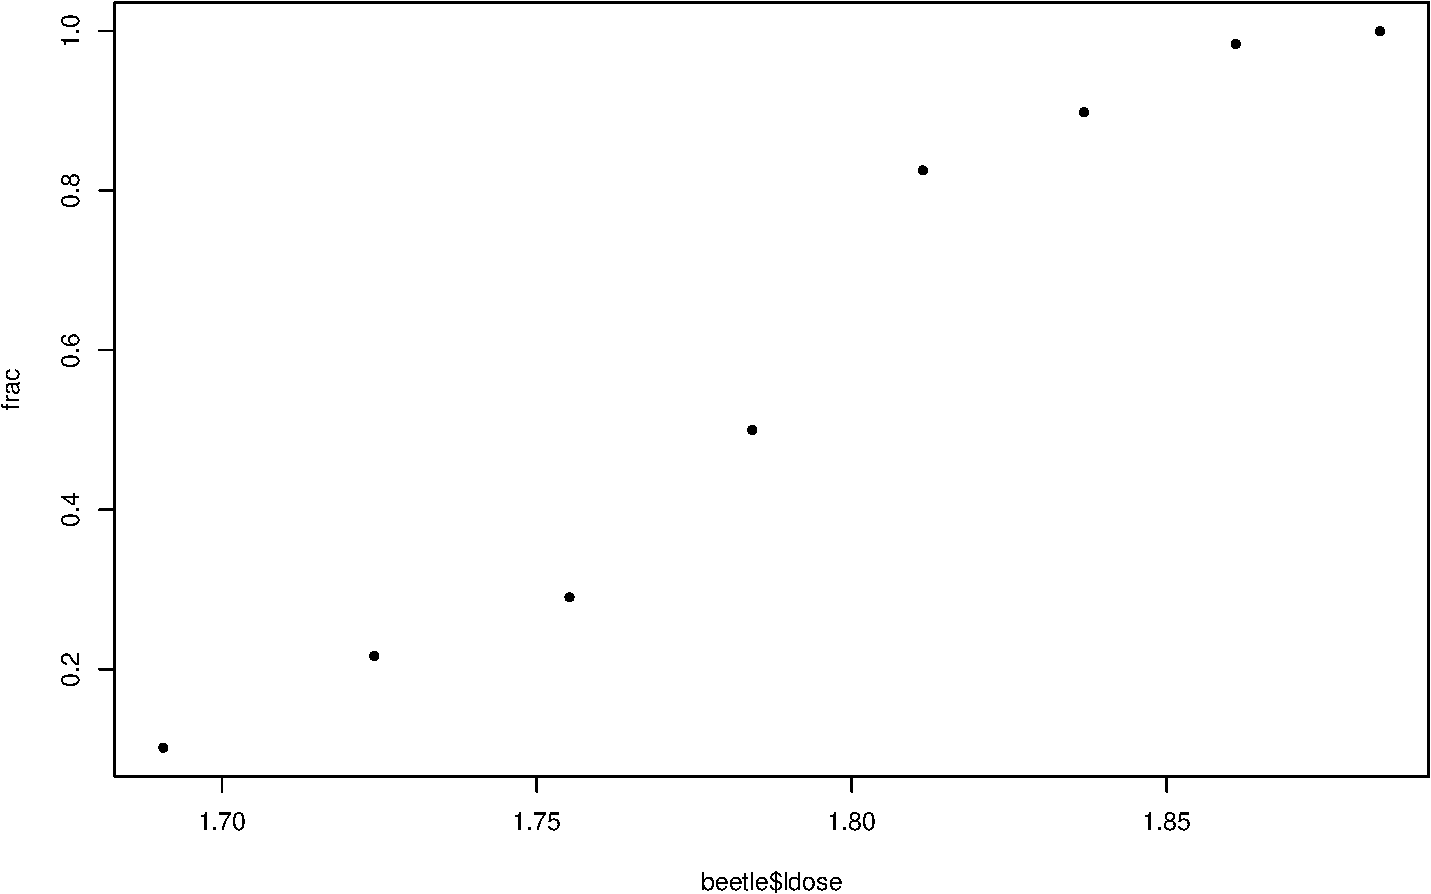
\includegraphics{1Intro_files/figure-beamer/beetles-1.pdf}
\end{block}
\end{block}
\end{frame}

\begin{frame}
What might be the distribution of the number of dead beetles, \(Y_i\) at
a given dose \(x_i\)? Dose \(x_i\) was given to \(n_i\) beetles.
\end{frame}

\begin{frame}
\[ Y_i=bin(n_i,\pi_i)\] where \(\pi_i\) =probability for a beetle to die
at dose \(x_i\) and \(n_i\)= number of beetles treated with dose
\(x_i\). A linear model for \(\pi_i\) estimated by ordinary least
squares is problematic because

\begin{itemize}
\item
  \(0 \le \pi_i \le 1\) can not be guaranteed by a linear expression
  \(\beta_0+\beta_1 x_i\), and
\item
  \(\text{Var}(Y_i) =n_i \pi_i (1-\pi_i)\) is non-constant
  (heteroscedastic) variance.
\end{itemize}
\end{frame}

\begin{frame}
The ``usual'' solution to this is \emph{logistic regression} where the
relationship between the mean of the response and the predictor is not
linear, but instead
\[ \ln(\frac{\pi_i}{1-\pi_i})= \beta_0+\beta_1 x_i \] or equivalently
\[\pi_i=\frac{\exp(\beta_0+\beta_1 x_i)}{1+\exp(\beta_0+\beta_1 x_i)}\]

Then \(0\le \pi_i\le 1\). We estimate the model by Maximum Likelihood
(ML), while taking into account that the responses are binomially
distributed.
\end{frame}

\begin{frame}[fragile]
\tiny

\begin{Shaded}
\begin{Highlighting}[]
\NormalTok{fit}\OtherTok{=}\FunctionTok{glm}\NormalTok{(}\FunctionTok{cbind}\NormalTok{(beetle}\SpecialCharTok{$}\NormalTok{y,beetle}\SpecialCharTok{$}\NormalTok{n}\SpecialCharTok{{-}}\NormalTok{beetle}\SpecialCharTok{$}\NormalTok{y)}\SpecialCharTok{\textasciitilde{}}\NormalTok{ldose,}\AttributeTok{data=}\NormalTok{beetle,}\AttributeTok{family=}\NormalTok{binomial)}
\FunctionTok{summary}\NormalTok{(fit)}
\end{Highlighting}
\end{Shaded}

\begin{verbatim}
## 
## Call:
## glm(formula = cbind(beetle$y, beetle$n - beetle$y) ~ ldose, family = binomial, 
##     data = beetle)
## 
## Deviance Residuals: 
##     Min       1Q   Median       3Q      Max  
## -1.5941  -0.3944   0.8329   1.2592   1.5940  
## 
## Coefficients:
##             Estimate Std. Error z value Pr(>|z|)    
## (Intercept)  -60.717      5.181  -11.72   <2e-16 ***
## ldose         34.270      2.912   11.77   <2e-16 ***
## ---
## Signif. codes:  0 '***' 0.001 '**' 0.01 '*' 0.05 '.' 0.1 ' ' 1
## 
## (Dispersion parameter for binomial family taken to be 1)
## 
##     Null deviance: 284.202  on 7  degrees of freedom
## Residual deviance:  11.232  on 6  degrees of freedom
## AIC: 41.43
## 
## Number of Fisher Scoring iterations: 4
\end{verbatim}

\normalsize
\end{frame}

\begin{frame}[fragile]
\tiny

\begin{Shaded}
\begin{Highlighting}[]
\NormalTok{thisrange}\OtherTok{=}\FunctionTok{range}\NormalTok{(beetle}\SpecialCharTok{$}\NormalTok{ldose)}
\NormalTok{xs}\OtherTok{=}\FunctionTok{seq}\NormalTok{(thisrange[}\DecValTok{1}\NormalTok{],thisrange[}\DecValTok{2}\NormalTok{],}\AttributeTok{length=}\DecValTok{100}\NormalTok{)}
\NormalTok{predicted}\OtherTok{=}\FunctionTok{predict}\NormalTok{(fit,}\AttributeTok{newdata=}\FunctionTok{data.frame}\NormalTok{(}\AttributeTok{ldose=}\NormalTok{xs),}\AttributeTok{type=}\StringTok{"response"}\NormalTok{)}
\FunctionTok{plot}\NormalTok{(beetle}\SpecialCharTok{$}\NormalTok{ldose,frac)}
\FunctionTok{lines}\NormalTok{(xs,predicted)}
\end{Highlighting}
\end{Shaded}

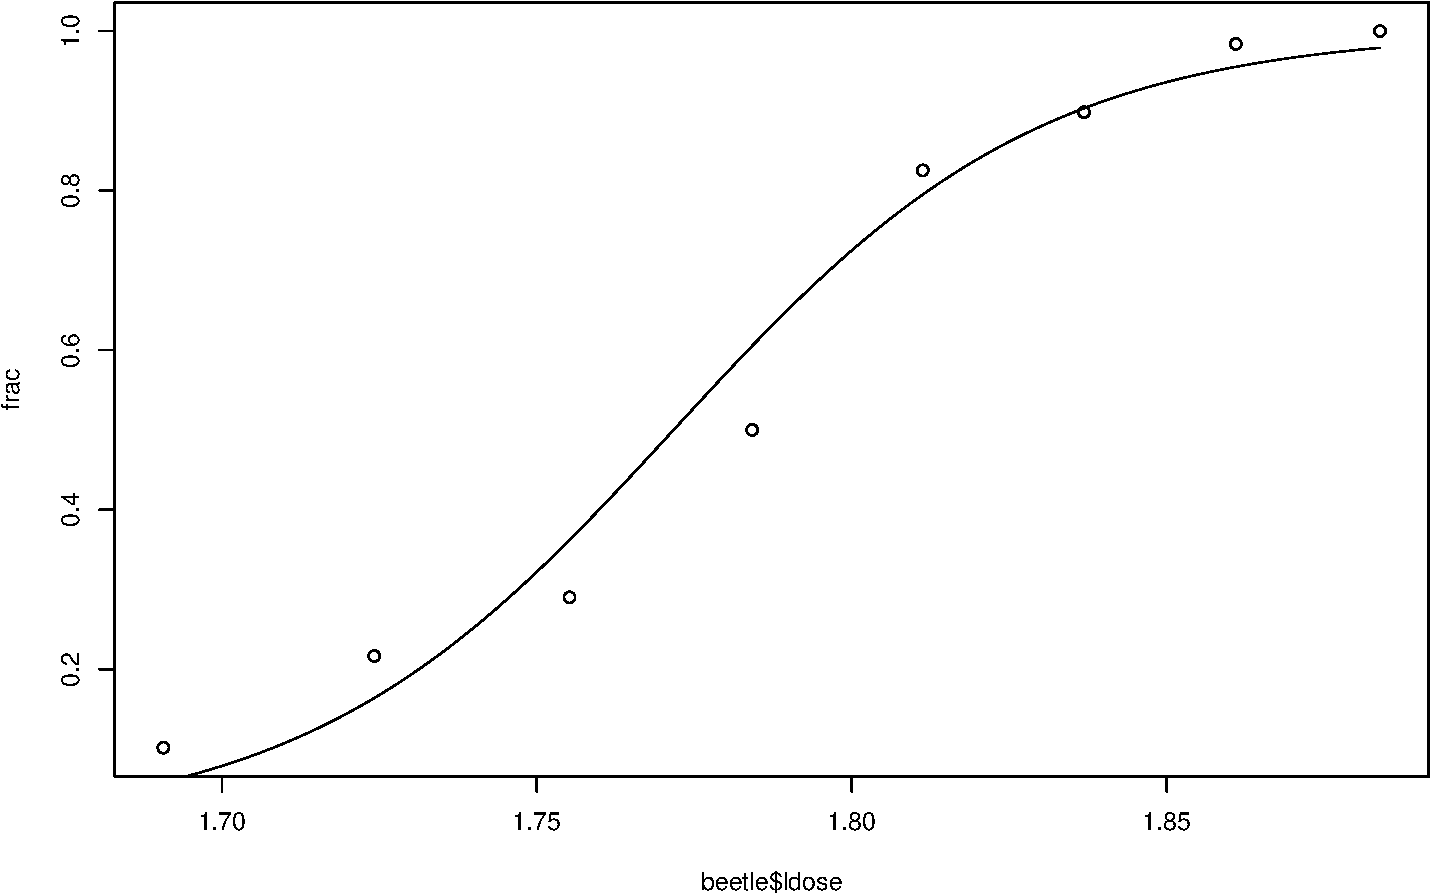
\includegraphics{1Intro_files/figure-beamer/unnamed-chunk-1-1.pdf}

\normalsize
\end{frame}

\begin{frame}
\textbf{PLAN:} In this module we will study the binary regression, work
on parameter estimation and interpretation of parameter estimates using
odds, work with both individual and grouped data, test linear
hypotheses, look at criteria for model fit and model choice, and discuss
overdispersion.

\textbf{Textbook:} 2.3 and 5.1.
\end{frame}

\begin{frame}[fragile]
\begin{block}{Module 4: Poisson and gamma regression}
\protect\hypertarget{module-4-poisson-and-gamma-regression}{}
Count data - the number of times and event occurs - is common. In one
famous study British doctors were in 1951 sent a questionnaire about
whether they smoked tobacco - and later information about their death
were collected. Questions that were asked were: Is the death rate higher
for smokers than for non-smokers? If so, by how much? And, how is this
related to age?

\tiny

\begin{Shaded}
\begin{Highlighting}[]
\FunctionTok{library}\NormalTok{(boot) }\CommentTok{\#n=person{-}year, ns=smoker{-}years, age=midpoint 10 year age group, }
\CommentTok{\#y=number of deaths due to cad, smoke=smoking status}
\FunctionTok{head}\NormalTok{(breslow,}\AttributeTok{n=}\DecValTok{10}\NormalTok{)}
\end{Highlighting}
\end{Shaded}

\begin{verbatim}
##    age smoke     n   y    ns
## 1   40     0 18790   2     0
## 2   50     0 10673  12     0
## 3   60     0  5710  28     0
## 4   70     0  2585  28     0
## 5   80     0  1462  31     0
## 6   40     1 52407  32 52407
## 7   50     1 43248 104 43248
## 8   60     1 28612 206 28612
## 9   70     1 12663 186 12663
## 10  80     1  5317 102  5317
\end{verbatim}

\normalsize
\end{block}
\end{frame}

\begin{frame}
To investigate this we will look at different ways of relating the
expected number of deaths and the number of doctors at risk in the
observation period for each smoke and age group. We will do this by
assuming a Poission distribution for the number of deaths, and linking
this to a linear predictor.

When we work with continuous data - like life times, costs and claim
sized - these may not be negative, and the their distribution often
follow a right skewed distribution. We will look at effect a one of more
covariates that may work multiplicative on the response and see how we
may fit that using gamma regression on the log scale of the response.

\textbf{Textbook:} 5.2 and 5.3
\end{frame}

\begin{frame}
\begin{block}{Module 5: GLM in general (and quasi likelihood --- if
time)}
\protect\hypertarget{module-5-glm-in-general-and-quasi-likelihood-if-time}{}
We will see that normal, binary, Poisson and gamma regression all have
the same underlying features:

\begin{enumerate}
\item
  The mean of the response, \(\mu_i=\text{E}(Y_i)\), is connected to the
  linear predictor \(\eta_i={\bf x}_i^T \beta\) by a link function:
  \(\eta_i=g(\mu_i)\) or, alternatively, by a response function
  \(\mu_i=h(\eta_i)\) - where \(g=h^{-1}\) (inverse functions).
\item
  The distribution of the response can be written as a univariate
  exponential family (we work with that in this first module).
\end{enumerate}

This leads to a unified framework, and maximum likelihood estimation can
be written on a generalized form for all the GLMs. In addition we can
present statistical inference and asymptotic properties of estimators on
a common form. Finally, we may expand this to quasi-likelihood models by
just specifying mean and variance (not distribution) and solve using
generalized estimation equations.
\end{block}
\end{frame}

\begin{frame}
This part is rather mathematical - but is built on the findings of
modules 1-4.

\textbf{Textbook:} 5.4 and 5.5
\end{frame}

\begin{frame}[fragile]
\begin{block}{Module 6: Categorical regression and contingency tables}
\protect\hypertarget{module-6-categorical-regression-and-contingency-tables}{}
Here our response variable has more than two categories, and these
categories can either be unordered or ordered. Examples of categorical
responses include (unordered) data in infection (no, or socalled type I
or type II) after Caesarian delivery, or (ordered) data on degree of
defoliation of trees (nine ordered categories).

We will use the multinomial distribution as the distribution for the
response, and work mainly with grouped data - that often can be
presented in a contingency table.

\tiny

\begin{Shaded}
\begin{Highlighting}[]
\NormalTok{ds}\OtherTok{=}\FunctionTok{read.table}\NormalTok{(}\StringTok{"https://www.math.ntnu.no/emner/TMA4315/2017h/data/caesarian.raw"}\NormalTok{,}\AttributeTok{header=}\ConstantTok{TRUE}\NormalTok{)}
\FunctionTok{head}\NormalTok{(ds)}
\end{Highlighting}
\end{Shaded}

\begin{verbatim}
##    n infbin RISK NPLAN ANTIB Y
## 1  0      1    1     0     1 1
## 2  1      1    1     0     1 2
## 3 17      0    1     0     1 3
## 4  0      1    0     0     1 1
## 5  0      1    0     0     1 2
## 6  2      0    0     0     1 3
\end{verbatim}

\normalsize
\end{block}
\end{frame}

\begin{frame}
For unordered categories (like the Caesarian delivery data) we will use
many logistic regressions - each between one category and a chosen
reference category. For ordered categories (like the defoliation of
trees) we will use a cumulative model, also called a proportional odds
model.
\end{frame}

\begin{frame}
If time permits we will also look briefly at exact and asymptotic
inference (Fishers exact test and Pearsons Chisquare test) for
contingency tables (unordered categories), which is closely related to
the GLM-presentation.

\textbf{Textbook:} Chapter 6, and possibly extra materiale on the Fisher
and Chi-square test (if time permits).

Compulsory exercise 2 will cover modules 3-6.
\end{frame}

\begin{frame}
\begin{block}{Module 7: Linear mixed effects models}
\protect\hypertarget{module-7-linear-mixed-effects-models}{}
In a study on the effect of sleep deprivation the average reaction time
per day were measured. On day 0 the subjects had their normal amount of
sleep. Starting that night they were restricted to 3 hours of sleep per
night. The observations represent the average reaction time on a series
of tests given each day to each subject. This was measured for 18
subjects for 10 days (days 0-9).
\end{block}
\end{frame}

\begin{frame}[fragile]
\tiny

\begin{Shaded}
\begin{Highlighting}[]
\FunctionTok{library}\NormalTok{(lme4)}
\FunctionTok{library}\NormalTok{(ggplot2) }\CommentTok{\# see more on ggplot later in this module}
\NormalTok{gg }\OtherTok{\textless{}{-}} \FunctionTok{ggplot}\NormalTok{(sleepstudy, }\FunctionTok{aes}\NormalTok{(}\AttributeTok{x =}\NormalTok{ Days, }\AttributeTok{y =}\NormalTok{ Reaction))}
\NormalTok{gg }\OtherTok{\textless{}{-}}\NormalTok{ gg }\SpecialCharTok{+} \FunctionTok{geom\_point}\NormalTok{(}\AttributeTok{color =} \StringTok{"blue"}\NormalTok{, }\AttributeTok{alpha =} \FloatTok{0.7}\NormalTok{)}
\NormalTok{gg }\OtherTok{\textless{}{-}}\NormalTok{ gg }\SpecialCharTok{+} \FunctionTok{geom\_smooth}\NormalTok{(}\AttributeTok{method =} \StringTok{"lm"}\NormalTok{, }\AttributeTok{color =} \StringTok{"black"}\NormalTok{)}
\NormalTok{gg }\OtherTok{\textless{}{-}}\NormalTok{ gg }\SpecialCharTok{+} \FunctionTok{theme\_bw}\NormalTok{()}
\NormalTok{gg }\OtherTok{\textless{}{-}}\NormalTok{ gg }\SpecialCharTok{+} \FunctionTok{facet\_wrap}\NormalTok{(}\SpecialCharTok{\textasciitilde{}}\NormalTok{Subject)}
\NormalTok{gg}
\end{Highlighting}
\end{Shaded}

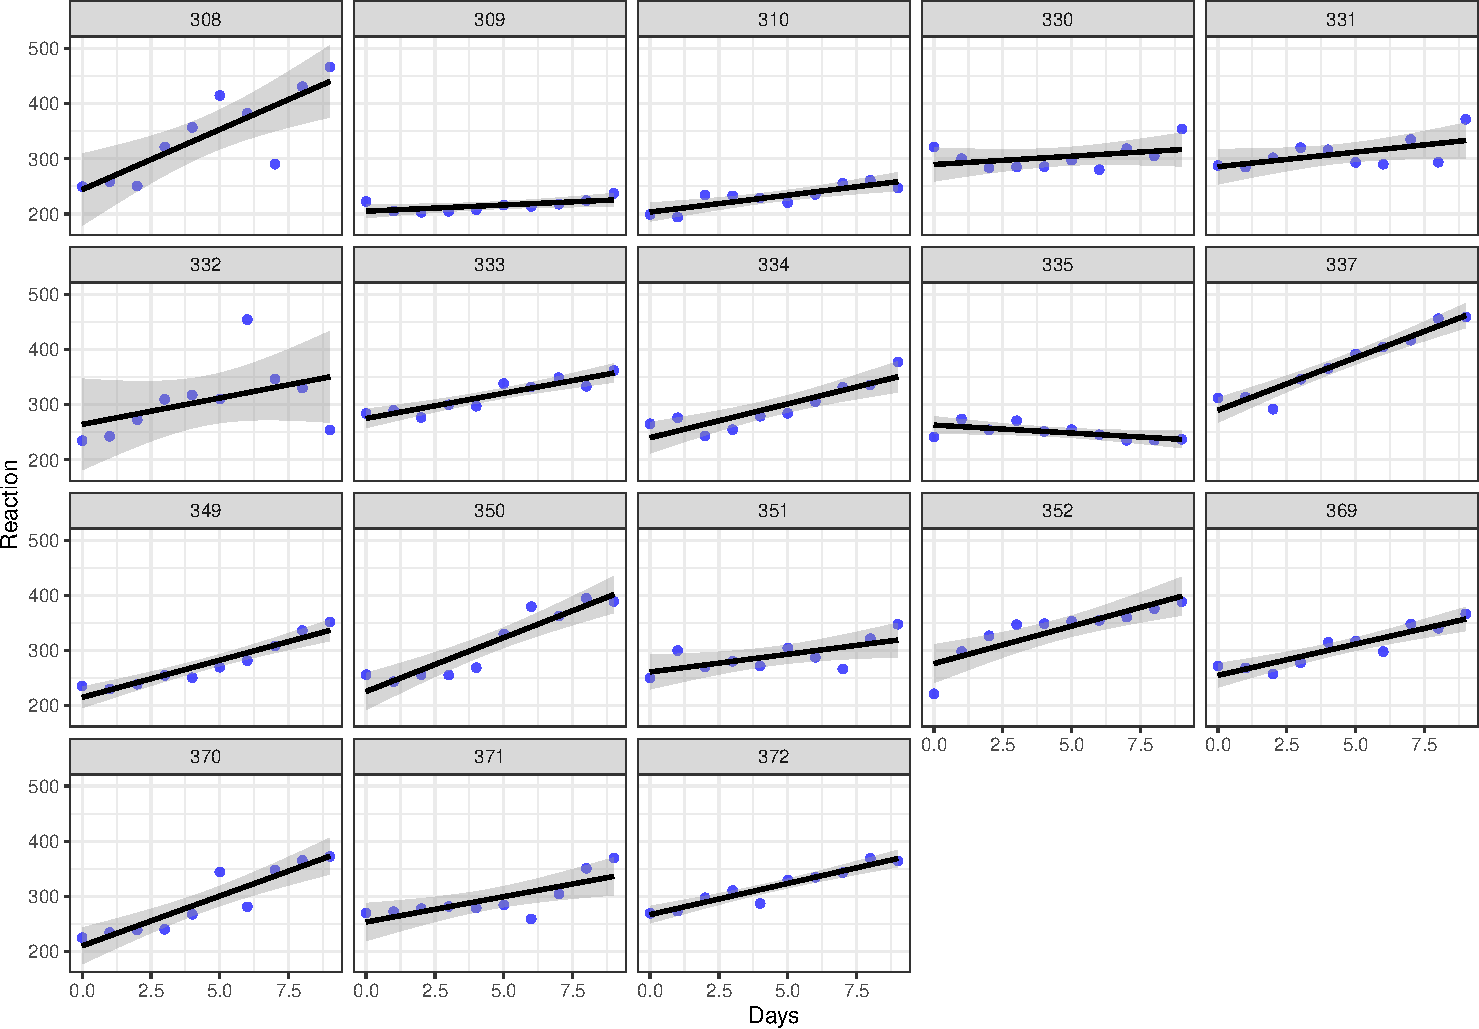
\includegraphics{1Intro_files/figure-beamer/unnamed-chunk-4-1.pdf}

\normalsize
\end{frame}

\begin{frame}
We observe that each subject's reaction time increases approximately
linearly with the number of sleepdeprived days. But, it appears that
subjects have different slopes and intercepts.

As a first model we may assume that there is a common intercept and
slope for the population - called fixed effects, but allow for random
deviations for the intercept and slope for each individual. In linear
mixed effects models we assume that the random intercepts and slopes are
drawn from normal distributions and estimate the variance in these
distribution. Such a model will make observations correlated within
subjects.
\end{frame}

\begin{frame}[fragile]
\tiny

\begin{Shaded}
\begin{Highlighting}[]
\NormalTok{fm1 }\OtherTok{\textless{}{-}} \FunctionTok{lmer}\NormalTok{(Reaction }\SpecialCharTok{\textasciitilde{}}\NormalTok{ Days }\SpecialCharTok{+}\NormalTok{ (Days }\SpecialCharTok{|}\NormalTok{ Subject), sleepstudy)}
\FunctionTok{summary}\NormalTok{(fm1)}
\end{Highlighting}
\end{Shaded}

\begin{verbatim}
## Linear mixed model fit by REML ['lmerMod']
## Formula: Reaction ~ Days + (Days | Subject)
##    Data: sleepstudy
## 
## REML criterion at convergence: 1743.6
## 
## Scaled residuals: 
##     Min      1Q  Median      3Q     Max 
## -3.9536 -0.4634  0.0231  0.4634  5.1793 
## 
## Random effects:
##  Groups   Name        Variance Std.Dev. Corr
##  Subject  (Intercept) 612.10   24.741       
##           Days         35.07    5.922   0.07
##  Residual             654.94   25.592       
## Number of obs: 180, groups:  Subject, 18
## 
## Fixed effects:
##             Estimate Std. Error t value
## (Intercept)  251.405      6.825  36.838
## Days          10.467      1.546   6.771
## 
## Correlation of Fixed Effects:
##      (Intr)
## Days -0.138
\end{verbatim}

\normalsize

Here the population fixed effects estimates are an intercept of 251.4 ms
and a slope of 10.47 ms/day. The random effects for the intercept and
the slope have estimated standard deviations 24.74 ms and 5.92 ms/day.
\end{frame}

\begin{frame}
In this module we will look at different models for clustered (schools,
families) and repeated measurement (e.g.~over time) using regression
with fixed and random effects.

\textbf{Textbook:} 2.4, 7.1, 7.3
\end{frame}

\begin{frame}
\begin{block}{Module 8: Generalized linear mixed effects models}
\protect\hypertarget{module-8-generalized-linear-mixed-effects-models}{}
We generalize our model in Module 7 - on normal responses - to binary
(and possibly Poisson) responses.

\textbf{Textbook:} 7.2, 7.5, 7.7

Compulsory exercise 3 will cover modules 7-8.
\end{block}

\begin{block}{Module 9: Discussion and conclusions}
\protect\hypertarget{module-9-discussion-and-conclusions}{}
\end{block}
\end{frame}

\begin{frame}
\begin{block}{Common - for all modules}
\protect\hypertarget{common---for-all-modules}{}
\begin{enumerate}
\item
  Model specification: an equation linking the response and the
  explanatory variables, and a probability distribution for the
  response.
\item
  Estimation of the parameters in the model
\item
  Checking the adequacy of the model, how well it fits the data.
\item
  Inference: confidence intervals, hypothesis tests, interpretation of
  results, prediction of future responses.
\end{enumerate}

Both theoretic derivations and practical analysis in R will be
emphasized.
\end{block}
\end{frame}

\begin{frame}{Learning outcome}
\protect\hypertarget{learning-outcome}{}
\textbf{Knowledge}.

The student can assess whether a generalised linear model can be used in
a given situation and can further carry out and evaluate such a
statistical analysis. The student has substantial knowledge of
generalised linear models and associated inference and evaluation
methods. This includes regression models for Gaussian distributed data,
logistic regression for binary and multinomial data, Poisson regression
and log-linear models for contingency tables.

The student has theoretical knowledge about linear mixed models and
generelized linear mixed effects models, and associated inference and
evaluation of the models. Main emphasis is on Gaussian and binomial
data.

\textbf{Skills}.

The student can assess whether a generalised linear model or a
generalized linear mixed model can be used in a given situation, and can
further carry out and evaluate such a statistical analysis.
\end{frame}

\begin{frame}{Learning styles}
\protect\hypertarget{learning-styles}{}
We (probably) all have different ways in which we learn - and we have
different learning ambitions when attending a course.

Back in 1988 Felder and Silverman published an article where they
suggested that there was a mismatch between the way students learn and
the way university courses were taught (in Science, Technology,
Engineering and Mathematics=STEM). They devised a taxonomy for learning
styles - where four different axis are defined:
\end{frame}

\begin{frame}
\begin{enumerate}
[1)]
\item
  \textbf{active - reflective}: How do you process information: actively
  (through physical activities and discussions), or reflexively (through
  introspection)?
\item
  \textbf{sensing-intuitive}: What kind of information do you tend to
  receive: sensitive (external agents like places, sounds, physical
  sensation) or intuitive (internal agents like possibilities, ideas,
  through hunches)?
\item
  \textbf{visual-verbal}: Through which sensorial channels do you tend
  to receive information more effectively: visual (images, diagrams,
  graphics), or verbal (spoken words, sound)?
\item
  \textbf{sequential - global}: How do you make progress: sequentially
  (with continuous steps), or globally (through leaps and an integral
  approach)?
\end{enumerate}

Here are a few words on the
\href{http://www4.ncsu.edu/unity/lockers/users/f/felder/public//ILSdir/styles.pdf}{four
axis}
\end{frame}

\begin{frame}
The idea in the 1988 article was that by \emph{acknowledging these
different learning style axes it was possible to guide the teachers to
choose teaching styles that matched the learning styles of the
students}. That is, many students (according to Felder and coauthors)
have a visual way of learning, and then teachers should spend time
devising visual aids (in addition to verbal aids - that were the
prominent aids in 1988), and so on.

\textbf{However, studies show that the students should use \emph{many}
different learning resources - not only one favourite (not only go to
plenary lectures or not only read in the book).}
\end{frame}

\begin{frame}
In this GLM course I have designed different learning resources, and
hope that many of these match your way of learning. To help me (and
maybe for you to get some insight into your own learning style)

\textbf{I ask you to answer a standardized set of questions made by
Felder et al (44 questions with two possible answers), and then report
your results to me in a Google form}.
\end{frame}

\begin{frame}
You can report your scores anonymously, or by giving our name. If you do
this anonymously I will have information on the class level, and if you
do this with your name I get to know a bit about how you learn and I can
use the results to help to construct student groups for the interactive
lectures. Your results will only be used by me, and I will not show them
to other people (students or staff). This means that this is not used
for research, but to increase the quality of the GLM course (in total
and for each one of you). I will never discuss your personal results in
class, but are very eager to discuss results on the class level - and
use these when designing new learning resources.

Here is the
\href{https://www.webtools.ncsu.edu/learningstyles/}{questionarie}
(maybe do a screen shot of your results -the results only appear on a
web page and is not saved or emailed to you or anyone).

I have taken the test and these were my results: I scored 3 on the
active side of the active-reflective scale, 1 on the sensing side of the
sensing-intuitive scale, 5 on the visual side on the visual-verbal scale
and finally 5 on the global side of the sequential-global scale. In the
Google form I would then report to have a ``active value'' for the
active-reflective axis, and then report the value to be 3. Then I would
choose ``sensing value'' on the sensoring-intuitive axis and report the
value to be 1, I will choose ``visual value'' and report 5, and finally
choose ``global value'' and report 5. (Values below 5 are reported to be
weak, and this means that there is no strong preference on that axis.)

Here is the \href{https://goo.gl/forms/p77EFhQabe9BIZT32}{Google form
where I ask that you write your 4 scores}

After you have submitted your scores please go back and read the
description of the four axis, but this time
\href{http://www4.ncsu.edu/unity/lockers/users/f/felder/public//ILSdir/styles.pdf}{focus
on the advice for the different type of learners}

If you are curios about the work of Felder and coauthors, more resources
can be found here: \url{http://educationdesignsinc.com/}
\end{frame}

\begin{frame}{Learning resources in the GLM course}
\protect\hypertarget{learning-resources-in-the-glm-course}{}
\#\#The module pages

I have divided the GLM course into modular units with specific focus, in
order to use smaller units (time and topic) to facilitate learning.

\begin{itemize}
\tightlist
\item
  The topic of each module on the agenda for 1---2 weeks of study.
\item
  All activity points to module pages.
\item
  Mathematics in LaTeX (also derivations present), figures and examples
  with R, all R code visible.
\end{itemize}
\end{frame}

\begin{frame}
\#\#\#Structure of module pages

\begin{enumerate}
[1)]
\tightlist
\item
  Introduction and aim
\item
  Motivating example
\item
  Theory---example loop
\item
  Recommended exercises
\item
  References, packages to install.
\end{enumerate}
\end{frame}

\begin{frame}
\begin{block}{How to use the module pages?}
\protect\hypertarget{how-to-use-the-module-pages}{}
\begin{itemize}
\tightlist
\item
  A slides version (output: beamer\_presentation) of the pages used in
  the plenary lectures.
\item
  A webpage version (output: html\_document) used in the (so-called)
  interactive lectures.
\item
  A document version (output: pdf\_document) used for student self
  study.
\item
  The Rmd version --- used as notebook to investigate changes to the R
  code.
\item
  Additional class notes (written in class) linked in.
\end{itemize}

The module pages are the backbone of the course!
\end{block}
\end{frame}

\begin{frame}
\textbf{Active students --- deep learning?} Since active students are
more able to analyse, evaluate and synthesise ideas?

\begin{itemize}
\tightlist
\item
  Provide learning environments, opportunities, interactions, tasks and
  instruction that foster deep learning.
\item
  Provide guidance and support that challenges students based on their
  current ability.
\item
  Students discover their current strengths and weaknesses and what they
  need to do to improve.
\end{itemize}

What are student active learing methods/tasks?

\begin{itemize}
\tightlist
\item
  Pause in plenary lecture to ask questions and let students think
  and/or discuss.
\item
  In-class quizzes (with the NTNU invention Kahoot!) --- individual and
  team mode.
\item
  Projects --- individual or in groups.
\item
  Group discussion.
\end{itemize}

Now: plenary and \emph{interactive lectures}.
\end{frame}

\begin{frame}
\#\#The plenary lectures (PL)

\begin{itemize}
\tightlist
\item
  for each module we start with a plenary lecture to introduce the aims,
\item
  use real data to examplify what to learn, why this is useful and what
  this is used in society
\item
  then we move to notation and focus on the model used
\item
  theory is then presented (writing - not slides), discussed and
\item
  mixed with use of R and data analysis.
\end{itemize}

The plenary lectures is rather passive in nature - for the students -
and held in classical auditorium. They provide the first step into the
new module.

\textbf{Q:} What are advantages of attending a plenary lecture (as
compared to reading the text book or the module pages, or watching
videoes)? Do you plan to attend the plenary lectures?
\end{frame}

\begin{frame}
\#\#The interactive lectures (IL)

has focus on student activity and understanding though discussing with
fellow students and with the lecturer/TA - in groups.

\begin{block}{Smia (the smithy)}
\protect\hypertarget{smia-the-smithy}{}
A room where interaction and activity is in focus. Flat floor with group
tables, whiteboard and screen --- PC and electricity outlets. 50
students.

\tiny \url{https://www.ntnu.no/laeringsarealer/smia}\normalsize
\end{block}
\end{frame}

\begin{frame}
\begin{enumerate}
\item
  Students arrive and are divided into groups (different criteria will
  be used). Short presentation round (name, study programme, interests)
  in the groups. One student (the ``manager'') log in to the PC at each
  table, or connect her/his own laptop and display the module page.
\item
  Lecturer gives a \emph{short} introduction to current state, and
  present a problem set (mainly exam problem).
\end{enumerate}
\end{frame}

\begin{frame}
\begin{enumerate}
\setcounter{enumi}{2}
\item
  Students work together in the group on the problem set. The problems
  are presented on the digital screen, and the students discuss by
  interacting around the screen and often by running (ready-made) R code
  and interpreting analysis output - all presented on the digital
  screen.
\item
  If the problem is of a theoretical flavour, or drawing is needed - the
  students work on the whiteboards next to the digital screen. One
  student may act as ``secretary''.
\end{enumerate}
\end{frame}

\begin{frame}
\begin{enumerate}
\setcounter{enumi}{4}
\item
  Lecturer summarizes solutions to the problem with input from the
  student groups.
\item
  This summarizing the first 45 minutes, then there is a break (with
  light refreshments) and then repeat 1-5 in the second hour.
\end{enumerate}

\textbf{More pictures of how the students in H2017 worked will be shown
in the PL.}
\end{frame}

\begin{frame}
\begin{block}{Statements from focus groups H2017}
\protect\hypertarget{statements-from-focus-groups-h2017}{}
(two groups of 4 students each, one hour ``interviews'' by external
evaluator - anonymous contributtions)

\#\#\#The concept

\textbf{Student A:} We are taught in a different way than what we have
experienced earlier --- sitting in groups, working on problem sets and
discussing. No, never experienced this before --- and we are master
students. Where was all this earlier?

\textbf{Student B:} It is very nice to have two hours every week to
discuss with the others, and be able to explain to each other and work
with the course material from a new point of view. We are not told what
is right, but we spend time finding that out --- together.

They also commented that the reading list was short and that they did
not think they had to prepare much for the exam --- they felt that they
really understood and were up to date.
\end{block}
\end{frame}

\begin{frame}
\#\#\#Learning outcome in group setting and new concepts

\textbf{Student C:} For most sessions I feel I learnt a lot. I remember
the concept we work on has been talked about in the plenary lectures,
and then I talk about the details with the others in the group and get
to explain to the others --- then I feel that I really know this
concept. I do not really learn so much new stuff, but I learn what we
have already gone through in the plenary lectures a lot better.

\textbf{Student D:} And, we get a confirmation that we have understood
what we were taught in the plenary lecture. Yes, I know this concept -
and so on - and I have not misunderstood - which may often happen. If I
have misunderstood I get corrected here in the interactive lecture -
this makes the learning more targeted (not so abstract).

\textbf{Student E:} Yes, I agree, what we learn becomes reinforced.
Personally I find it hard to learn new concepts in a group setting.

Comment: hard to come to IL if not up-to-date on reading list (e.g.~not
read by yourself or attended PL).
\end{frame}

\begin{frame}
\begin{block}{But, they were also worried:}
\protect\hypertarget{but-they-were-also-worried}{}
\textbf{Student F:} I believe Mette cannot go so deep in the plenary
lecture - compared to when we had the double amount of plenary lectures.
She plans for us to learn by ourselves, which I think is a good thing. I
beleive that we have a greater gain from learning together, and from
seeing each others problems, and we learn from each other.

\textbf{Student G:} I agree, I think it is more challenging for a
lecturer to divide the course in interactive and plenary lectures than
only using plenary lectures. The lecturer needs to teach in two
different ways, but also to try to cover all material in effectively
shorter time. Maybe this results in us loosing the depth understanding,
maybe that is how it is, and that is sad.

This was the main motivation behind the module pages --- having the full
story written out, but choosing parts to present in the plenary lectures
and parts in the interactive lectures.
\end{block}
\end{frame}

\begin{frame}
\textbf{Questions:}

\begin{itemize}
\tightlist
\item
  Who are the interactive lectures for?
\item
  What are advantages of attending an interactive lecture?
\item
  When you finish your studies and head for a job - go you think the
  skills developed in the interactive lectures will be in demand?
\item
  Do you think the interactive lectures will be challenging for you to
  attend? Why?
\item
  How can the lecturer help you make this easier? Personal adjustment
  can be made.
\item
  If the IL worked well in 2017, does it mean that it will also work in
  2018?
\end{itemize}
\end{frame}

\begin{frame}
\#\#The compulsory exercises

has mainly focus on programming and interpretation - with some theory -
and can be worked on in small groups (1-3). Will be a test of acquired
understanding, and will constitute 30\% of the final evaluation.
\end{frame}

\begin{frame}{Practical details}
\protect\hypertarget{practical-details}{}
go to Blackboard \href{https://innsida.ntnu.no/bb-student}{student
log-in} or
\href{https://ntnu.blackboard.com/webapps/login?action=guest_login\&new_loc=/webapps/blackboard/execute/courseMain?course_id=_11002_1}{guest
access}.
\end{frame}

\begin{frame}{Core concept: Exponential family of distributions}
\protect\hypertarget{core-concept-exponential-family-of-distributions}{}
\end{frame}

\begin{frame}
In this course we will look at models where the distribution of the
response variable, \(y_i\), can be written in the form of a
\emph{univariate exponential family}
\[ f(y_i\mid \theta_i)=\exp \left( \frac{y_i \theta_i-b(\theta_i)}{\phi}\cdot w_i + c(y_i, \phi, w_i) \right) \]
where

\begin{itemize}
\item
  \(\theta_i\) is called the canonical parameter and is a parameter of
  interest
\item
  \(\phi\) is called a nuisance parameter (and is not of interest to
  us=therefore a nuisance (plage))
\item
  \(w_i\) is a weight function, in most cases \(w_i=1\)
\item
  b and c are known functions.
\end{itemize}

It can be shown that \(\text{E}(Y_i)=b'(\theta_i)\) and
\(\text{Var}(Y_i)=b''(\theta_i)\cdot \frac{\phi}{w}\).

Remark: slightly different versions of writing the exponential family
exists, but we will use this version in our course (a different version
might be used in TMA4295, but the basic findings are the same).
\end{frame}

\begin{frame}{Interactive lectures - problem set}
\protect\hypertarget{interactive-lectures---problem-set}{}
You may of cause read through the problem set before the interactive
lecture, but that is not a prerequisite. Solutions will be provided to
the major part of the recommended exercises (but not to the R-part of
this one).

\begin{block}{Theoretical questions (first hour)}
\protect\hypertarget{theoretical-questions-first-hour}{}
We will work with the exponential family, but to make the notation
easier for these tasks, we omit the \(i\) subscript.

\[ f(y \mid \theta)=\exp \left( \frac{y \theta-b(\theta)}{\phi}\cdot w + c(y, \phi, w) \right) \]

\#\#\#Problem 1: Choose (discuss and then talk to lecturer/TA) if you
will work on a) binomial, b) Poisson, c) univariate normal or d) gamma.
\end{block}
\end{frame}

\begin{frame}
\begin{enumerate}
[a)]
\tightlist
\item
  What process can produce a \(Y\) that is binomially distributed? Write
  down the probability mass function, f(x). Is the binomial distribution
  an the exponential family? Identify \(b\) and \(c\) and show the
  connection with the mean and variance of \(Y\).
\end{enumerate}

NB: you may first use \(n=1\) in the binomial (which then is called
Bernoulli) - since that is much easier than a general \(n\).

Hint: \url{https://wiki.math.ntnu.no/tma4245/tema/begreper/discrete} and
nearly the same parameterization for showing the binomial is member of
exponential \url{https://www.youtube.com/watch?v=7mNrsFr7P_A}.

\begin{enumerate}
[a)]
\setcounter{enumi}{1}
\tightlist
\item
  What about the Poisson distribution? What process can produce a \(Y\)
  that is Poisson distributed? Write down the probability mass function,
  f(x). Is the Poisson distribution an the exponential family? Identify
  \(b\) and \(c\) and show the connection with the mean and variance of
  \(Y\).
\end{enumerate}

Hint: \url{https://wiki.math.ntnu.no/tma4245/tema/begreper/discrete} and
first part of
\href{https://mediasite.ntnu.no/Mediasite/Play/db9c6fbc45bf48abb8a4dd00ff146e081d?catalog=0fce6173-7a98-4db7-84b7-50cba3a3a341}{Sannsynlighetsmaksimering}
\end{frame}

\begin{frame}
\begin{enumerate}
[a)]
\setcounter{enumi}{2}
\item
  What about the (univariate) normal? What process can produce a \(Y\)
  that is normally distributed? Write down the probability distribution
  function, f(x). Is the univariate normal distribution an the
  exponential family? Identify \(b\) and \(c\) and show the connection
  with the mean and variance of \(Y\).
\item
  What about the gamma distribution? What process can produce a \(Y\)
  that is gamma distributed? There are many different parameterizations
  for the gamma pdf, and we will use this (our textbook page 643):
  \(Y \sim Ga(\mu,\nu)\) with density
  \[ f(y)=\frac{1}{\Gamma(\nu)} (\frac{\nu}{\mu})^{\nu} y^{\nu-1}\exp(-\frac{\nu}{\mu}y) \text{ for }y>0\]
\end{enumerate}

Is the gammadistribution an the exponential family? Identify \(b\) and
\(c\) and show the connection with the mean and variance of \(Y\).

Hint: \url{https://wiki.math.ntnu.no/tma4245/tema/begreper/continuous}
\end{frame}

\begin{frame}
\#\#\#Problem 2. Choose either alternative a or b.

Alternative a: Prove that \(\text{E}(Y_i)=b'(\theta_i)\) and
\(\text{Var}(Y_i)=b''(\theta_i)\cdot \frac{\phi}{w}\). Hint: integration
by parts, and investigate what is
\(\int_{-\infty}^{\infty} \frac{df}{dy}dy\)?

Alternative b: The following is a derivation of the mean and variance of
an exponential family. Go through this derivation and specify why you go
from one step to another.
\href{https://www.math.ntnu.no/emner/TMA4315/2017h/M5ExpFamProofEVar.pdf}{Derivation}
\end{frame}

\begin{frame}[fragile]
\begin{block}{Exam questions with the exponential family -- optional
(covered above)}
\protect\hypertarget{exam-questions-with-the-exponential-family-optional-covered-above}{}
We have covered the Poisson and gamma in the problem sets above, but not
the negative binomial (not in the core of the course)

\begin{block}{Exam December 2017, Problem 1a: Poisson regression}
\protect\hypertarget{exam-december-2017-problem-1a-poisson-regression}{}
(Remark: last question can not be answered before module 4.)

Consider a random variable \(Y\). In our course we have considered the
univariate exponential family having distribution (probability density
function for continuous variables and probability mass function for
discrete variables)
\[ f(y)=\exp(\frac{y \theta +b(\theta)}{\phi}w + c(y,\phi,w))\] where
\(\theta\) is called the \emph{natural parameter} (or parameter of
interest) and \(\phi\) the \emph{dispersion parameter}.

The Poisson distribution is a discrete distribution with probability
mass function
\[ f(y)=\frac{\lambda^{y}}{y!}\exp(- \lambda), \text{ for } y=0,1,...,\]
where \(\lambda>0\).

\textbf{a}) {[}10 points{]}

Show that the Poisson distribution is a univariate exponential family,
and specify what are the elements of the exponential family
\((\theta,\phi,b(\theta),w,c(y,\phi,w))\).

What is the connection between \(\text{E}(Y)\) and the elements of the
exponential family?

What is the connection between \(\text{Var}(Y)\) and the elements of the
exponential family?

Use these connections to derive the mean and variance for the Poisson
distribution.

If the Poisson distribution is used as the distribution for the response
in a generalized linear model, what is then the \emph{canonical link}
function?
\end{block}

\begin{block}{Exam 2012, Problem 3: Precipitation in Trondheim, amount}
\protect\hypertarget{exam-2012-problem-3-precipitation-in-trondheim-amount}{}
Remark: the text is slightly modified from the original exam since we
parameterized the gamma as in our textbook.

We want to model the amount of daily precipitation given that it
\emph{is} precipitation, and denote this quantity \(Y\). It is common to
model \(Y\) as a gamma distributed random variable,
\(Y \sim Gamma(\nu,\mu)\), with density

\[ f_Y(y) = \frac{1}{\Gamma(\nu)} \left(\frac{\nu}{\mu}\right)^{\nu} y^{\nu-1}\exp\left(-\frac{\nu}{\mu} y \right) \]

In this problem we consider \(N\) observations, each gamma distributed
with \(Y_i \sim Gamma(\nu, \mu_i)\) (remark: common \(\nu\)). Here
\(\nu\) is considered to be a known nuisance parameter, and the
\(\mu_i\)s are unknown.

\textbf{a)} Show that the gamma distribution function is member of the
exponential family when \(\mu_i\) is the parameter of interest.\\
Use this to find expressions for the expected value and the variance of
\(Y_i\), in terms of \((\nu,\mu_i)\), and interpret \(\nu\).
\end{block}

\begin{block}{Exam 2010, Problem 2: Negative binomial distribution}
\protect\hypertarget{exam-2010-problem-2-negative-binomial-distribution}{}
The probability density function for a negative binomial random variable
is
\[f_y(y; \theta, r) = \frac{\Gamma(y + r)}{y! \Gamma(r)} (1-\theta)^r \theta^y\]
for \(y = 0,1,2,\ldots,\), \(r>0\) and \(\theta \in (0,1)\), and where
\(\Gamma()\) denotes the gamma function. (There are also other
parameterizations of the negative binomial distributions, but use this
for now.)

\textbf{a)} Show that the negative binomial distribution is an
exponential family. You can in this question consider \(r\) as a known
constant.

\textbf{b)} Use the general formulas for a exponential family to show
that \(\text{E}(Y)=\mu=r\frac{\theta}{1-\theta}\) and
\(\text{Var}(Y)=\mu \frac{1}{1-\theta}\).
\end{block}
\end{block}

\begin{block}{Focus on R-related topics (second hour)}
\protect\hypertarget{focus-on-r-related-topics-second-hour}{}
\end{block}

\begin{block}{R, Rstudio, CRAN and GitHub - and R Markdown}
\protect\hypertarget{r-rstudio-cran-and-github---and-r-markdown}{}
\begin{block}{What is R?}
\protect\hypertarget{what-is-r}{}
\url{https://www.r-project.org/about.html}
\end{block}

\begin{block}{What is Rstudio?}
\protect\hypertarget{what-is-rstudio}{}
\url{https://www.rstudio.com/products/rstudio/}
\end{block}

\begin{block}{What is an R package?}
\protect\hypertarget{what-is-an-r-package}{}
\url{http://r-pkgs.had.co.nz} (We will make an R package in the exercise
part of this course.)
\end{block}

\begin{block}{What is CRAN?}
\protect\hypertarget{what-is-cran}{}
\url{https://cran.uib.no/}
\end{block}

\begin{block}{What is GitHub and Bitbucket?}
\protect\hypertarget{what-is-github-and-bitbucket}{}
Do we need GitHub or Bitbucket in our course?
\url{https://www.youtube.com/watch?v=w3jLJU7DT5E} and
\url{https://techcrunch.com/2012/07/14/what-exactly-is-github-anyway/}
\end{block}

\begin{block}{What is R Markdown?}
\protect\hypertarget{what-is-r-markdown}{}
\url{http://r4ds.had.co.nz/r-markdown.html}
\end{block}

\begin{block}{What is \texttt{knitr}?}
\protect\hypertarget{what-is-knitr}{}
\url{https://yihui.name/knitr/}
\end{block}

\begin{block}{What is R Shiny?}
\protect\hypertarget{what-is-r-shiny}{}
\url{https://shiny.rstudio.com/}

(In the statistics group we will build R Shiny app for the thematic
pages for our TMA4240/TMA4245/ST1101/ST1201/ST0103 introductory courses,
so if you have ideas for cool graphical presentation please let us know
- we have some economical resources available for help from master
students in statistics! Also ideas for this GLM course is or interest!)

The IMF R Shiny server is here: \url{https://shiny.math.ntnu.no/} (not
anything there now, but a lot more soooon).

(Remember the test you did to brush up on R programming?
\url{https://tutorials.shinyapps.io/04-Programming-Basics/\#section-welcome}
This was made with a combination of the R package \texttt{learnr} and a
shiny server.)
\end{block}
\end{block}
\end{frame}

\begin{frame}[fragile]
\begin{block}{Explore R Markdown in Rstudio}
\protect\hypertarget{explore-r-markdown-in-rstudio}{}
Quotations from
\url{https://rmarkdown.rstudio.com/authoring_quick_tour.html}:

\begin{itemize}
\tightlist
\item
  Creating documents with R Markdown starts with an .Rmd file that
  contains a combination of markdown (content with simple text
  formatting) and R code chunks.
\item
  The .Rmd file is fed to knitr, which executes all of the R code chunks
  and creates a new markdown (.md) document which includes the R code
  and it's output.
\item
  The markdown file generated by knitr is then processed by pandoc which
  is responsible for creating a finished web page, PDF, MS Word
  document, slide show, handout, book, dashboard, package vignette or
  other format.
\end{itemize}

The module pages (you are reading the Module 1 page now), are written
using R Markdown. To work with the module pages you either copy-paste
snippets of R code from the module page over in your editor window in
Rstudio, or copy the Rmd-version of the module page (1Intro.Rmd) into
your Rstudio editor window (then you can edit directly in Rmarkdown
document - to make it into your personal copy).

If you choose the latter: To compile the R code we use \texttt{knitr}
(termed ``knit'') to produce a html-page you press ``knit'' in menu of
the editor window, but first you need to install packages:
\texttt{rmarkdown} and \texttt{devtools} (from CRAN). For the module
pages the needed R packages will always be listed in the end of the
module pages.

If you want to learn more about the R Markdown (that you may use for the
compulsory exercises) this is a good read:

\begin{itemize}
\item
  \url{http://r4ds.had.co.nz/r-markdown.html} (Chapter 27: R Markdown
  from the ``R for Data Science'' book), and
\item
  the Rstudio cheat sheet on R Markdown is here:
  \url{https://www.rstudio.com/wp-content/uploads/2016/03/rmarkdown-cheatsheet-2.0.pdf}.
\end{itemize}

Then you see that you can make a pdf-file in addition to a html-file
(for your reports you may choose either). To make the pdf-file you need
latex to be installed on your machine.
\end{block}

\begin{block}{Not use R Markdown, but only R code?}
\protect\hypertarget{not-use-r-markdown-but-only-r-code}{}
If you only want to extract the R code from a R Markdown file you may do
that using the function \texttt{purl} from library \texttt{knitr}. To
produce a file ``1Intro.R'' from this ``1Intro.Rmd'' file:

\begin{Shaded}
\begin{Highlighting}[]
\FunctionTok{library}\NormalTok{(knitr)}
\FunctionTok{purl}\NormalTok{(}\StringTok{"https://www.math.ntnu.no/emner/TMA4315/2018h/1Intro.Rmd"}\NormalTok{)}
\end{Highlighting}
\end{Shaded}

The file will then be saved in your working directory, that you see with
\texttt{getwd()}.
\end{block}
\end{frame}

\begin{frame}[fragile]
\begin{block}{R packages}
\protect\hypertarget{r-packages}{}
And to work with either the 1Intro.R or 1Intro.Rmd file you will have to
first install the following libraries:

\begin{Shaded}
\begin{Highlighting}[]
\FunctionTok{install.packages}\NormalTok{(}\FunctionTok{c}\NormalTok{(}\StringTok{"rmarkdown"}\NormalTok{,}\StringTok{"gamlss.data"}\NormalTok{,}\StringTok{"tidyverse"}\NormalTok{,}\StringTok{"ggpubr"}\NormalTok{,}\StringTok{"investr"}\NormalTok{,}\StringTok{"lme4"}\NormalTok{))}
\end{Highlighting}
\end{Shaded}

For the subsequent module pages this information will be available in
the end of the page.
\end{block}
\end{frame}

\begin{frame}[fragile]
\begin{block}{The Munic Rent Index Data set}
\protect\hypertarget{the-munic-rent-index-data-set}{}
We will use this data set when working with multiple linear regression
(next module), so this is a good way to start to know the data set and
the ggplot functions, which can be installed together with a suite of
useful libraries from \texttt{tidyverse}.

A version of the Munic Rent Index data is available as \texttt{rent} in
library \texttt{catdata} from CRAN.

\begin{Shaded}
\begin{Highlighting}[]
\FunctionTok{library}\NormalTok{(gamlss.data)}
\FunctionTok{library}\NormalTok{(ggplot2)}
\end{Highlighting}
\end{Shaded}

Get to know the \texttt{rent} data.

\begin{Shaded}
\begin{Highlighting}[]
\NormalTok{ds}\OtherTok{=}\NormalTok{rent99}
\FunctionTok{colnames}\NormalTok{(ds)}
\end{Highlighting}
\end{Shaded}

\begin{verbatim}
## [1] "rent"     "rentsqm"  "area"     "yearc"    "location" "bath"     "kitchen" 
## [8] "cheating" "district"
\end{verbatim}

\begin{Shaded}
\begin{Highlighting}[]
\FunctionTok{dim}\NormalTok{(ds)}
\end{Highlighting}
\end{Shaded}

\begin{verbatim}
## [1] 3082    9
\end{verbatim}

\begin{Shaded}
\begin{Highlighting}[]
\FunctionTok{summary}\NormalTok{(ds)}
\end{Highlighting}
\end{Shaded}

\begin{verbatim}
##       rent            rentsqm             area            yearc      location
##  Min.   :  40.51   Min.   : 0.4158   Min.   : 20.00   Min.   :1918   1:1794  
##  1st Qu.: 322.03   1st Qu.: 5.2610   1st Qu.: 51.00   1st Qu.:1939   2:1210  
##  Median : 426.97   Median : 6.9802   Median : 65.00   Median :1959   3:  78  
##  Mean   : 459.44   Mean   : 7.1113   Mean   : 67.37   Mean   :1956           
##  3rd Qu.: 559.36   3rd Qu.: 8.8408   3rd Qu.: 81.00   3rd Qu.:1972           
##  Max.   :1843.38   Max.   :17.7216   Max.   :160.00   Max.   :1997           
##  bath     kitchen  cheating    district   
##  0:2891   0:2951   0: 321   Min.   : 113  
##  1: 191   1: 131   1:2761   1st Qu.: 561  
##                             Median :1025  
##                             Mean   :1170  
##                             3rd Qu.:1714  
##                             Max.   :2529
\end{verbatim}

Then, head for plotting with \texttt{ggplot} but first take a quick look
at the \texttt{ggplot2} library:

\begin{itemize}
\tightlist
\item
  Grolemund and Hadwick (2017): ``R for Data Science'', Chapter 3:
  Visualisation: \url{http://r4ds.had.co.nz/data-visualisation.html}
\end{itemize}

Before you continue you should have read the start of the Visualisation
chapter that explains the ggplot grammar. Yes, you start with creating
the coordinate system with \texttt{ggplot} and then add layers. What
does the following words mean: mapping, aesthetic, geom function mean in
the \texttt{ggplot} setting?

\begin{itemize}
\tightlist
\item
  The Rstudio cheat sheet on ggplot2 is here:
  \url{https://www.rstudio.com/wp-content/uploads/2016/11/ggplot2-cheatsheet-2.1.pdf}
\end{itemize}

First, look at plotting \texttt{rentsqm} for different values of
\texttt{location} - with panels of scatter plots and with boxplots

\begin{Shaded}
\begin{Highlighting}[]
\FunctionTok{ggplot}\NormalTok{(}\AttributeTok{data=}\NormalTok{ds)}\SpecialCharTok{+}
  \FunctionTok{geom\_point}\NormalTok{(}\AttributeTok{mapping=}\FunctionTok{aes}\NormalTok{(area,rentsqm))}\SpecialCharTok{+}
  \FunctionTok{facet\_wrap}\NormalTok{(}\SpecialCharTok{\textasciitilde{}}\NormalTok{location,}\AttributeTok{nrow=}\DecValTok{1}\NormalTok{)}
\end{Highlighting}
\end{Shaded}

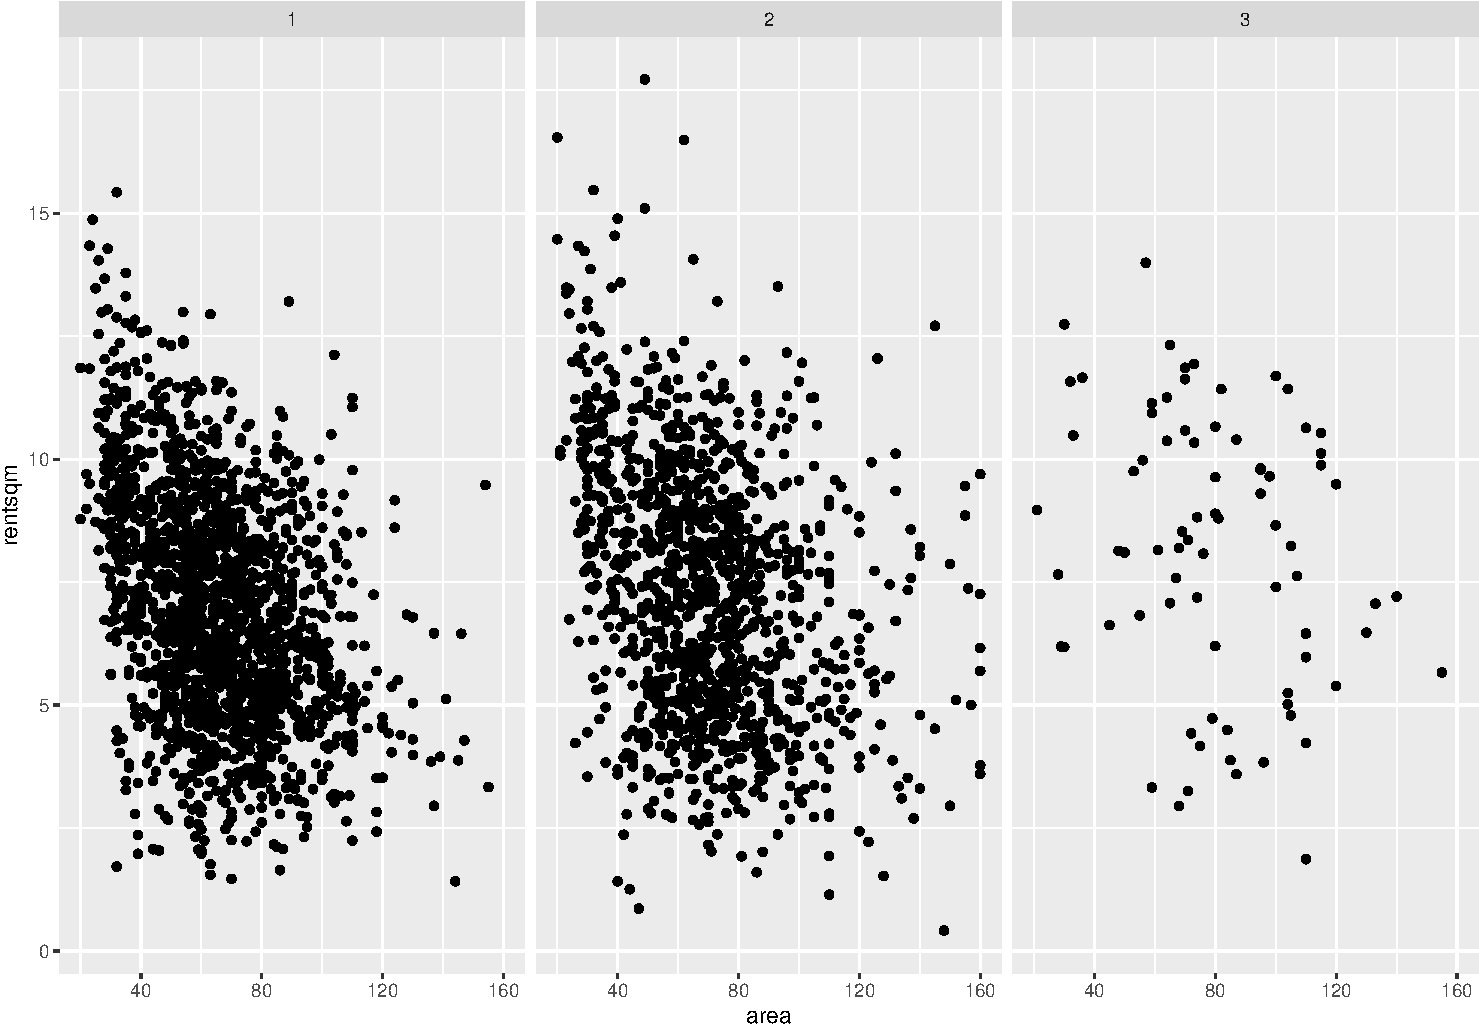
\includegraphics{1Intro_files/figure-beamer/unnamed-chunk-9-1.pdf}

\begin{Shaded}
\begin{Highlighting}[]
\FunctionTok{ggplot}\NormalTok{(}\AttributeTok{data =}\NormalTok{ ds, }\AttributeTok{mapping =} \FunctionTok{aes}\NormalTok{(}\AttributeTok{x =}\NormalTok{ location, }\AttributeTok{y =}\NormalTok{ rentsqm)) }\SpecialCharTok{+} 
  \FunctionTok{geom\_boxplot}\NormalTok{()}
\end{Highlighting}
\end{Shaded}

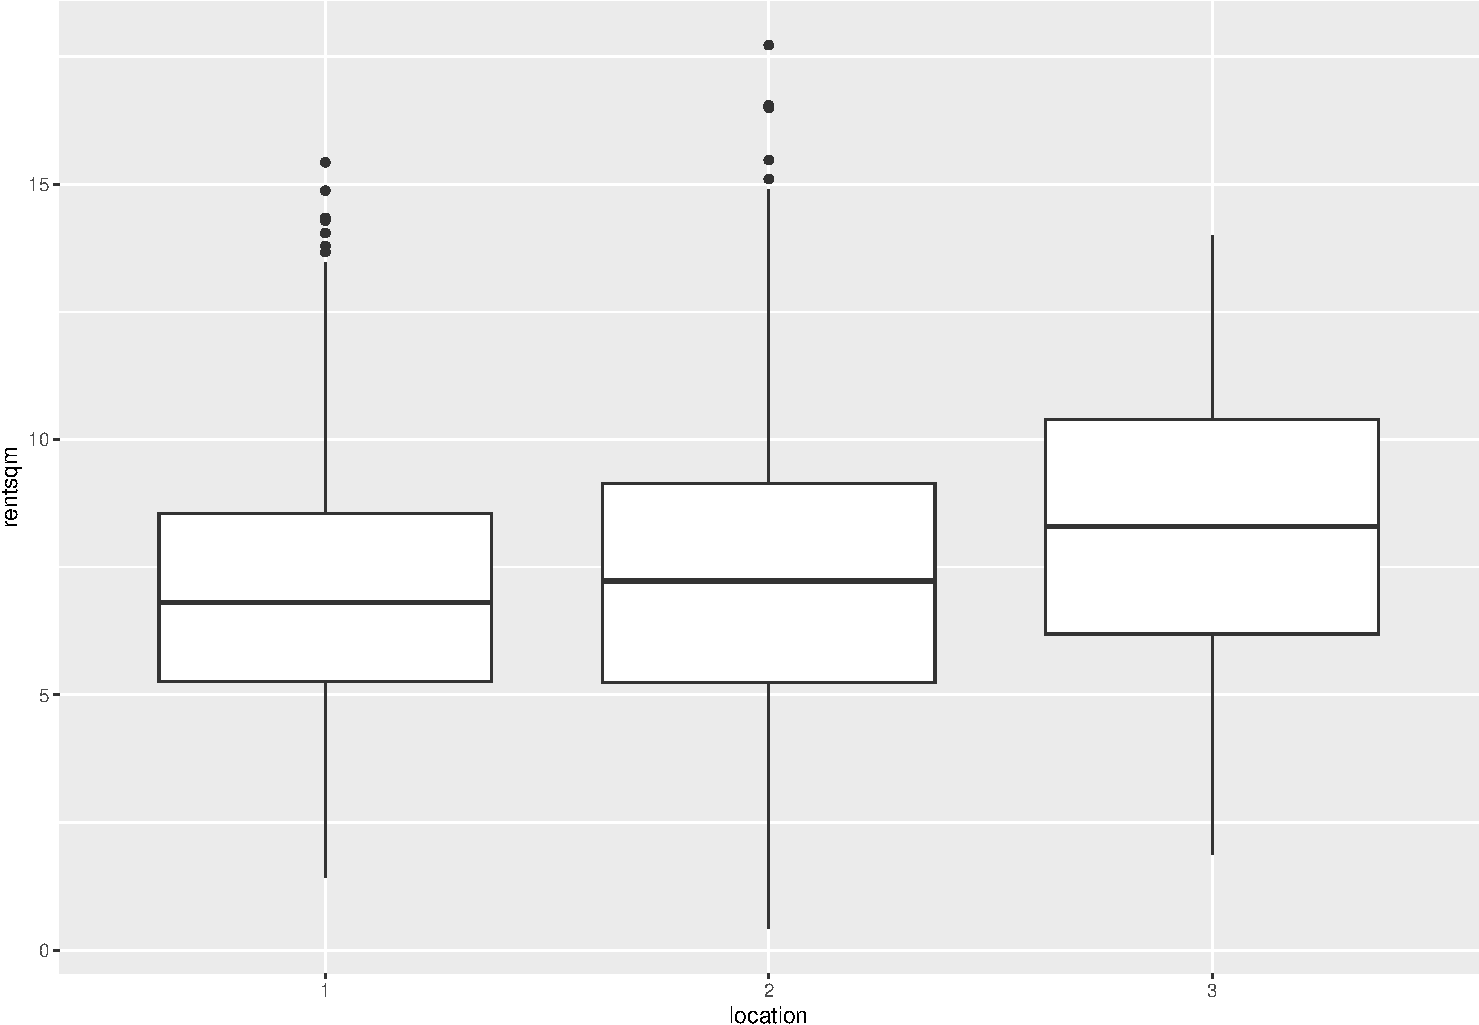
\includegraphics{1Intro_files/figure-beamer/unnamed-chunk-9-2.pdf}

So, location matters.

But, should we use \texttt{rent} or \texttt{rentsqm} as response?

\begin{Shaded}
\begin{Highlighting}[]
\FunctionTok{library}\NormalTok{(ggpubr)}
\NormalTok{plot1 }\OtherTok{\textless{}{-}} \FunctionTok{ggplot}\NormalTok{(}\AttributeTok{data=}\NormalTok{ds) }\SpecialCharTok{+}
  \FunctionTok{geom\_density}\NormalTok{(}\AttributeTok{mapping=}\FunctionTok{aes}\NormalTok{(rent),}\AttributeTok{kernel=}\StringTok{"gaussian"}\NormalTok{)}
\NormalTok{plot2 }\OtherTok{\textless{}{-}} \FunctionTok{ggplot}\NormalTok{(}\AttributeTok{data=}\NormalTok{ds) }\SpecialCharTok{+}
  \FunctionTok{geom\_density}\NormalTok{(}\AttributeTok{mapping=}\FunctionTok{aes}\NormalTok{(rentsqm),}\AttributeTok{kernel=}\StringTok{"gaussian"}\NormalTok{)}
\FunctionTok{ggarrange}\NormalTok{(plot1, plot2, }\AttributeTok{ncol=}\DecValTok{2}\NormalTok{)}
\end{Highlighting}
\end{Shaded}

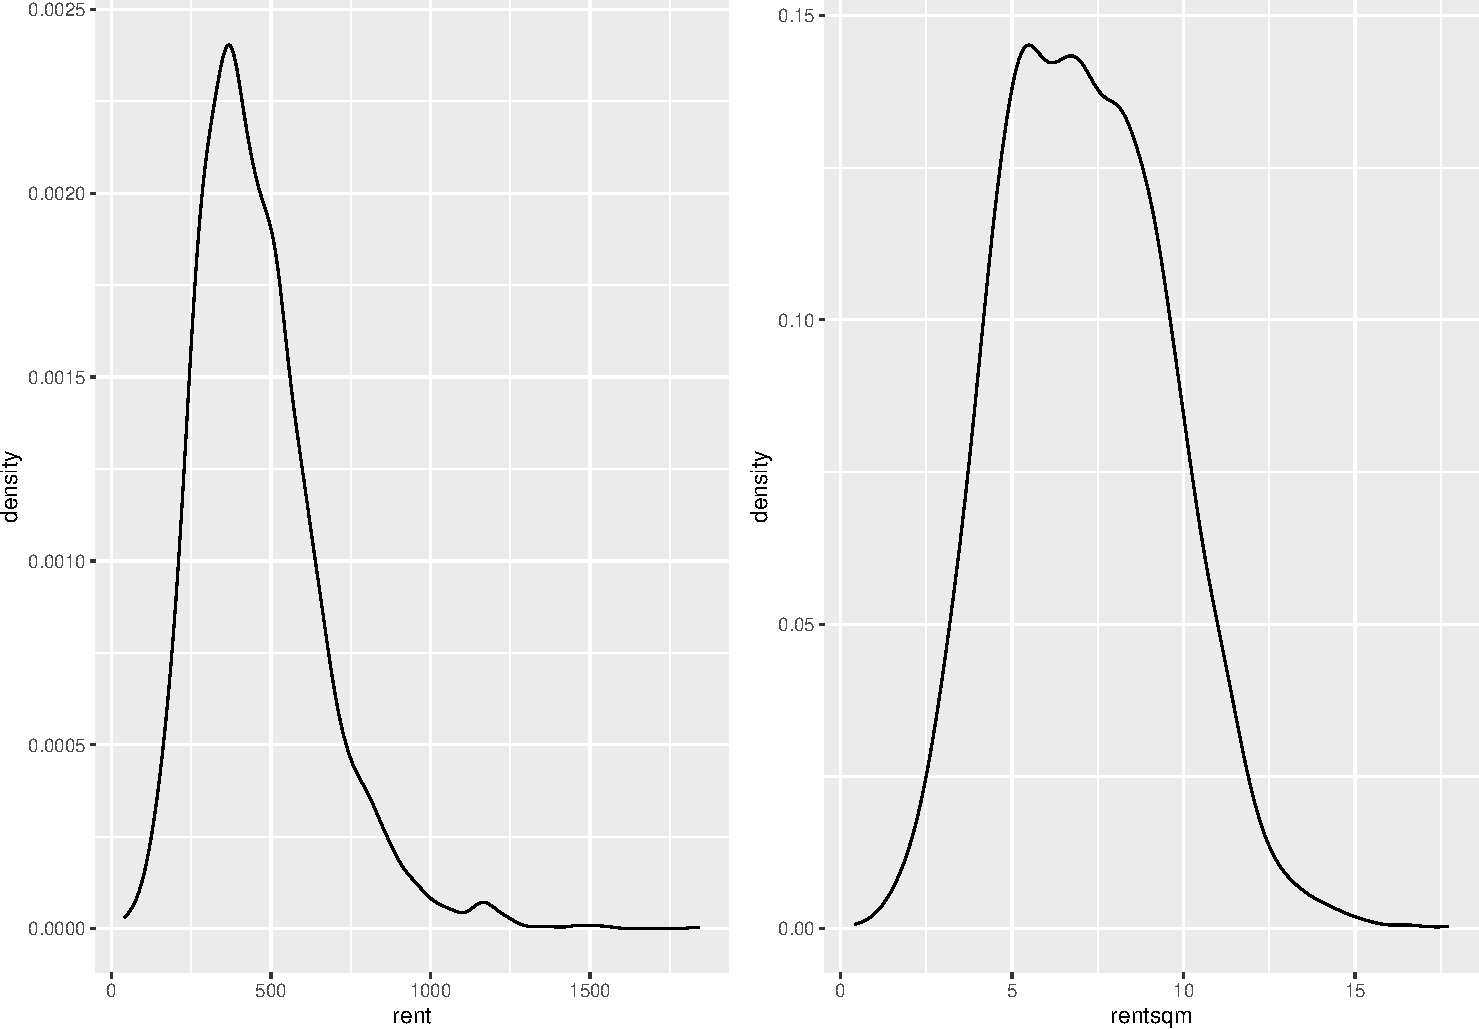
\includegraphics{1Intro_files/figure-beamer/unnamed-chunk-10-1.pdf}

So, which response will we use? And, what if we would include
\texttt{area} as covariate? I have plotted two plots together below,
more on mixing graphs on the same page (we need ggprbr, gridExtra and
cowplot packages)
\url{https://www.r-bloggers.com/ggplot2-easy-way-to-mix-multiple-graphs-on-the-same-page/}

Relationship between \texttt{rent} or \texttt{rentsqm} and \texttt{area}

\begin{Shaded}
\begin{Highlighting}[]
\NormalTok{plot1 }\OtherTok{\textless{}{-}} \FunctionTok{ggplot}\NormalTok{(}\AttributeTok{data=}\NormalTok{ds,}\FunctionTok{aes}\NormalTok{(area,rent))}\SpecialCharTok{+}
  \FunctionTok{geom\_point}\NormalTok{(}\AttributeTok{mapping=}\FunctionTok{aes}\NormalTok{(area,rent),}\AttributeTok{size=}\FloatTok{0.5}\NormalTok{)}
\NormalTok{plot2 }\OtherTok{\textless{}{-}} \FunctionTok{ggplot}\NormalTok{(}\AttributeTok{data=}\NormalTok{ds)}\SpecialCharTok{+}
  \FunctionTok{geom\_point}\NormalTok{(}\AttributeTok{mapping=}\FunctionTok{aes}\NormalTok{(area,rentsqm),}\AttributeTok{size=}\FloatTok{0.5}\NormalTok{)}
\FunctionTok{ggarrange}\NormalTok{(plot1, plot2, }\AttributeTok{ncol=}\DecValTok{2}\NormalTok{)}
\end{Highlighting}
\end{Shaded}

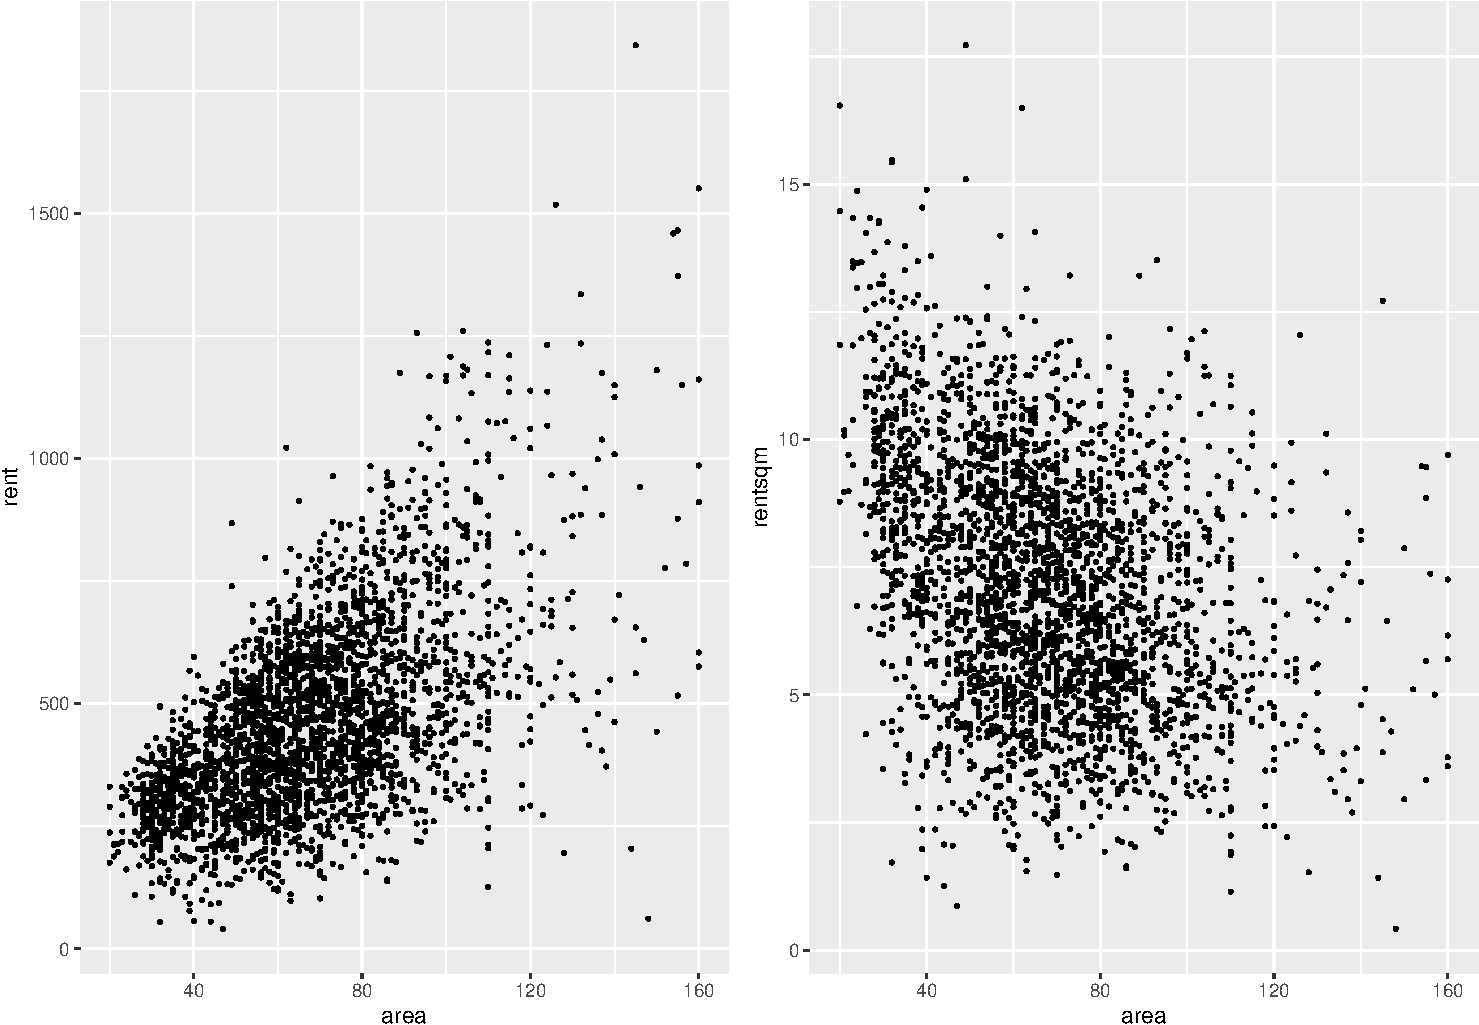
\includegraphics{1Intro_files/figure-beamer/unnamed-chunk-11-1.pdf}

So, if we include area as a covariate, we may look at residuals when
using \texttt{rent} or \texttt{rentsqm}. More about diagnostic plots in
Module 2 - but - which plot below looks more random?

\begin{Shaded}
\begin{Highlighting}[]
\NormalTok{lm.rent}\OtherTok{=}\FunctionTok{lm}\NormalTok{(rent}\SpecialCharTok{\textasciitilde{}}\NormalTok{area,}\AttributeTok{data=}\NormalTok{ds)}
\FunctionTok{summary}\NormalTok{(lm.rent)}
\end{Highlighting}
\end{Shaded}

\begin{verbatim}
## 
## Call:
## lm(formula = rent ~ area, data = ds)
## 
## Residuals:
##     Min      1Q  Median      3Q     Max 
## -786.63 -104.88   -5.69   95.93 1009.68 
## 
## Coefficients:
##             Estimate Std. Error t value Pr(>|t|)    
## (Intercept) 134.5922     8.6135   15.63   <2e-16 ***
## area          4.8215     0.1206   39.98   <2e-16 ***
## ---
## Signif. codes:  0 '***' 0.001 '**' 0.01 '*' 0.05 '.' 0.1 ' ' 1
## 
## Residual standard error: 158.8 on 3080 degrees of freedom
## Multiple R-squared:  0.3417, Adjusted R-squared:  0.3415 
## F-statistic:  1599 on 1 and 3080 DF,  p-value: < 2.2e-16
\end{verbatim}

\begin{Shaded}
\begin{Highlighting}[]
\NormalTok{lm.rentsqm}\OtherTok{=}\FunctionTok{lm}\NormalTok{(rentsqm}\SpecialCharTok{\textasciitilde{}}\NormalTok{area,}\AttributeTok{data=}\NormalTok{ds)}
\FunctionTok{summary}\NormalTok{(lm.rentsqm)}
\end{Highlighting}
\end{Shaded}

\begin{verbatim}
## 
## Call:
## lm(formula = rentsqm ~ area, data = ds)
## 
## Residuals:
##     Min      1Q  Median      3Q     Max 
## -6.9622 -1.5737 -0.1102  1.5861  9.9674 
## 
## Coefficients:
##             Estimate Std. Error t value Pr(>|t|)    
## (Intercept)  9.46883    0.12426   76.20   <2e-16 ***
## area        -0.03499    0.00174  -20.11   <2e-16 ***
## ---
## Signif. codes:  0 '***' 0.001 '**' 0.01 '*' 0.05 '.' 0.1 ' ' 1
## 
## Residual standard error: 2.291 on 3080 degrees of freedom
## Multiple R-squared:  0.1161, Adjusted R-squared:  0.1158 
## F-statistic: 404.5 on 1 and 3080 DF,  p-value: < 2.2e-16
\end{verbatim}

\begin{Shaded}
\begin{Highlighting}[]
\NormalTok{p1}\OtherTok{\textless{}{-}}\FunctionTok{ggplot}\NormalTok{(lm.rent, }\FunctionTok{aes}\NormalTok{(.fitted, .resid))}\SpecialCharTok{+}\FunctionTok{geom\_point}\NormalTok{()}
\NormalTok{p1}\OtherTok{\textless{}{-}}\NormalTok{p1}\SpecialCharTok{+}\FunctionTok{stat\_smooth}\NormalTok{(}\AttributeTok{method=}\StringTok{"loess"}\NormalTok{)}\SpecialCharTok{+}\FunctionTok{geom\_hline}\NormalTok{(}\AttributeTok{yintercept=}\DecValTok{0}\NormalTok{, }\AttributeTok{col=}\StringTok{"red"}\NormalTok{, }\AttributeTok{linetype=}\StringTok{"dashed"}\NormalTok{)}
\NormalTok{p1}\OtherTok{\textless{}{-}}\NormalTok{p1}\SpecialCharTok{+}\FunctionTok{xlab}\NormalTok{(}\StringTok{"Fitted values"}\NormalTok{)}\SpecialCharTok{+}\FunctionTok{ylab}\NormalTok{(}\StringTok{"Residuals"}\NormalTok{)}
\NormalTok{p1}\OtherTok{\textless{}{-}}\NormalTok{p1}\SpecialCharTok{+}\FunctionTok{ggtitle}\NormalTok{(}\StringTok{"Rent: Residual vs Fitted Plot"}\NormalTok{)}\SpecialCharTok{+}\FunctionTok{theme\_bw}\NormalTok{()}
\NormalTok{p2}\OtherTok{\textless{}{-}}\FunctionTok{ggplot}\NormalTok{(lm.rentsqm, }\FunctionTok{aes}\NormalTok{(.fitted, .resid))}\SpecialCharTok{+}\FunctionTok{geom\_point}\NormalTok{()}
\NormalTok{p2}\OtherTok{\textless{}{-}}\NormalTok{p2}\SpecialCharTok{+}\FunctionTok{stat\_smooth}\NormalTok{(}\AttributeTok{method=}\StringTok{"loess"}\NormalTok{)}\SpecialCharTok{+}\FunctionTok{geom\_hline}\NormalTok{(}\AttributeTok{yintercept=}\DecValTok{0}\NormalTok{, }\AttributeTok{col=}\StringTok{"red"}\NormalTok{, }\AttributeTok{linetype=}\StringTok{"dashed"}\NormalTok{)}
\NormalTok{p2}\OtherTok{\textless{}{-}}\NormalTok{p2}\SpecialCharTok{+}\FunctionTok{xlab}\NormalTok{(}\StringTok{"Fitted values"}\NormalTok{)}\SpecialCharTok{+}\FunctionTok{ylab}\NormalTok{(}\StringTok{"Residuals"}\NormalTok{)}
\NormalTok{p2}\OtherTok{\textless{}{-}}\NormalTok{p2}\SpecialCharTok{+}\FunctionTok{ggtitle}\NormalTok{(}\StringTok{"rentsqm: Residual vs Fitted Plot"}\NormalTok{)}\SpecialCharTok{+}\FunctionTok{theme\_bw}\NormalTok{()}
\FunctionTok{ggarrange}\NormalTok{(p1, p2, }\AttributeTok{ncol=}\DecValTok{2}\NormalTok{)}
\end{Highlighting}
\end{Shaded}

\begin{verbatim}
## `geom_smooth()` using formula = 'y ~ x'
## `geom_smooth()` using formula = 'y ~ x'
\end{verbatim}

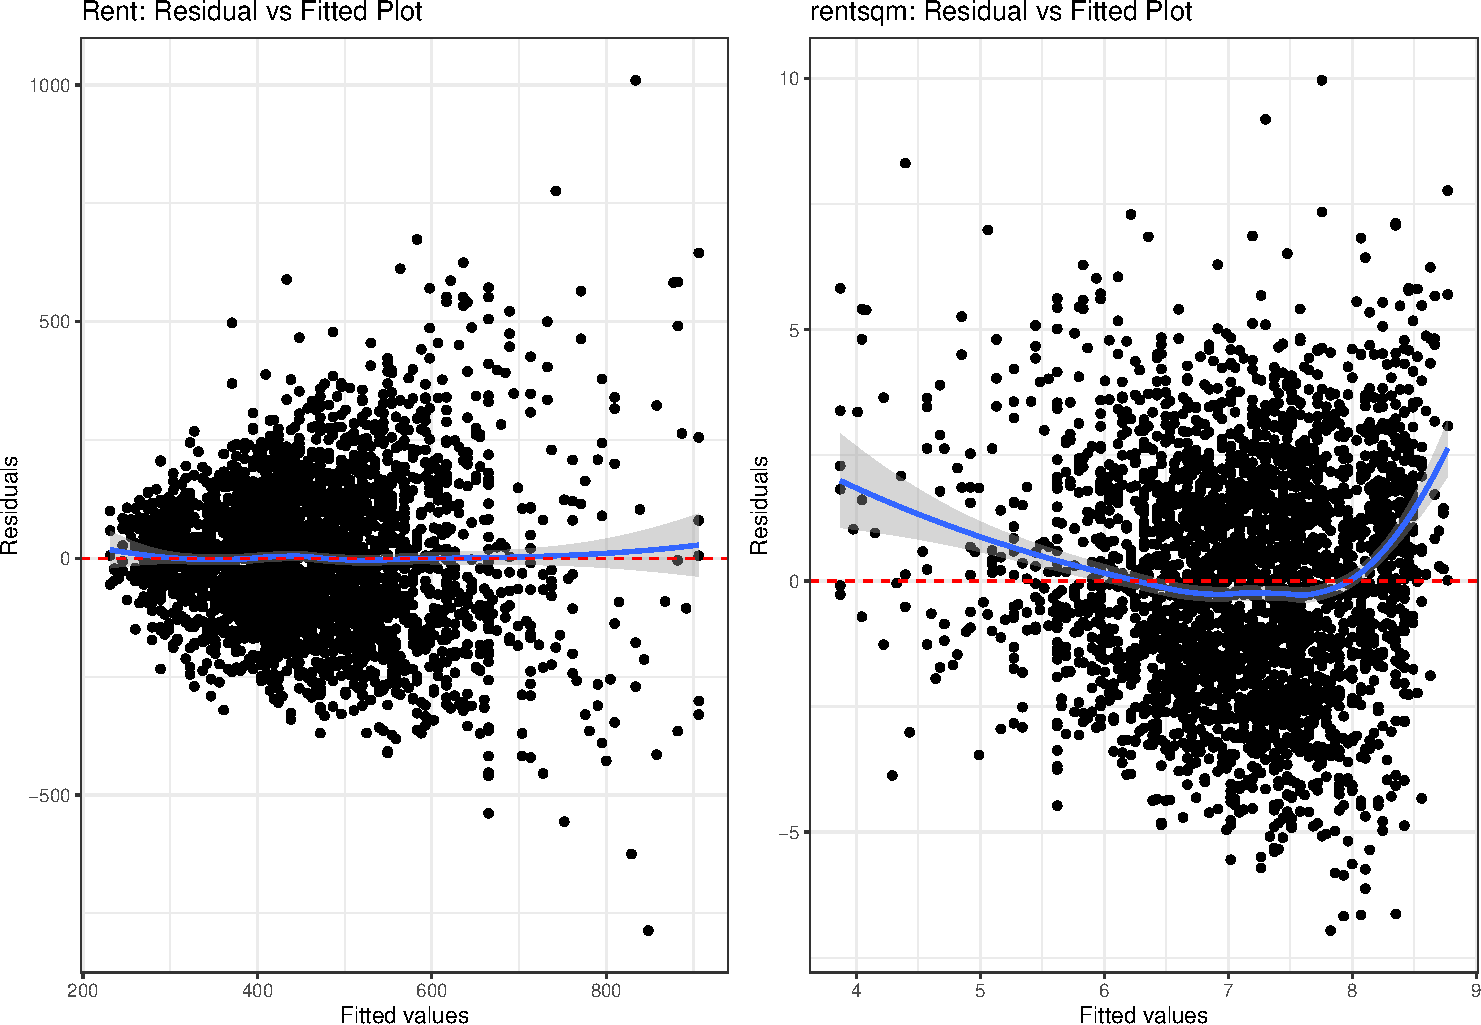
\includegraphics{1Intro_files/figure-beamer/unnamed-chunk-12-1.pdf}

Take home message: for the mean of the response may differ with out
covariates - that is why we use regression. For the normal linear
regression it is not the response that is supposed to have mean zero,
but the error term - more about this in Module 2. And, is the variance
of the residuals independent of the fitted values? Yes, more in Module
2.
\end{block}
\end{frame}

\begin{frame}
\begin{block}{Combining exercise 1 and 2:}
\protect\hypertarget{combining-exercise-1-and-2}{}
Choose one of the distributions you studied earlier (binomial, Poisson,
normal or gamma), and write a R-markdown document answering the
questions on requirements, f(x), f(x) as exponential family and mean and
variance. Also add R-code to plot f(x) and F(x) for a given set of
parameters - and add the mean as a vertical line - using the ggplot
library. Submit your Rmd document to the lecturer (email) - so it can be
added to this module solutions, or make your own github repository and
email the link to your repo to be added to this module page.
\end{block}
\end{frame}

\begin{frame}{Further reading}
\protect\hypertarget{further-reading}{}
\begin{itemize}
\item
  Grolemund and Hadwick (2017): ``R for Data Science'',
  \url{http://r4ds.had.co.nz}
\item
  Xie, Allaire and Grolemund (2018): ``R Markdown --- the definitive
  guide'', \url{https://bookdown.org/yihui/rmarkdown/}
\item
  Hadwick (2009):
  \href{https://link.springer.com/book/10.1007\%2F978-0-387-98141-3}{``ggplot2:
  Elegant graphics for data analysis'' textbook}.
\item
  Wilkinson (2005):
  \href{https://www.springer.com/gp/book/9780387245447}{The grammar of
  graphics}. The theory behind the ggplot2 package universe.
\item
  If you want to see more of the powers of ggplot, combined with a nice
  story:
  \url{https://www.andrewheiss.com/blog/2017/08/10/exploring-minards-1812-plot-with-ggplot2/}
\item
  R-bloggers: \url{https://https://www.r-bloggers.com/} is a good place
  to look for tutorials.
\item
  Stack Overflow: \url{https://stackoverflow.com/} is a good place to
  look for answers to your R questions (but also try the GLM teaching
  team)
\end{itemize}
\end{frame}

\end{document}
